\documentclass{article}
\usepackage{graphicx}
\usepackage{verbatim}
\usepackage{dcolumn}
\usepackage{array}
\usepackage{mathtools}
\usepackage{float}
\usepackage{booktabs}
\usepackage{cleveref}
\usepackage{siunitx}
\usepackage{enumitem}
\usepackage{bbm}
\usepackage{xcolor}
\usepackage{amsmath}
\usepackage{amsfonts}
\usepackage{amsthm}
\usepackage{amssymb}
\usepackage{booktabs}
\usepackage{caption}
\usepackage{float}
\usepackage{natbib}
\newtheorem{assump}{Assumption}[section]
\newtheorem{lemma}{Lemma}[section]
\newtheorem{corollary}{Corollary}[section]
\newtheorem{theorem}{Theorem}[section]
\usepackage[toc,page]{appendix}
\pagestyle{plain}
\topmargin 0.0cm
\oddsidemargin 0.2cm
\textwidth 16cm
\textheight 21cm
\footskip 1.0cm
\title{A Dynamic Panel Data Framework for Identification and Estimation of Nonlinear Production Functions}
\author{Justin Doty\thanks{Department of Economics, University of Iowa, S321 Pappajohn Business Building, 21 E Market St, Iowa City, IA 52242. Email: \texttt{justin-doty@uiowa.edu}}
}
\date{\vspace{-5ex}}
\begin{document}
\maketitle{}

\begin{abstract}
This paper studies identification and estimation of a non-linear model for production functions with unobserved heterogeneity. Non-parametric identification results are established for the production function under stationarity assumptions. This paper then estimates the conditional quantiles of firm production using non-linear quantile regression. This paper finds that objects of interest, such as output elasticities with respect to inputs vary considerably with respect to the rank of unobserved technology shocks. In the application to US firm-level manufacturing data, this paper considers a Translog production function with non-Hicksian neutral productivity shocks and a productivity process that features non-linear persistence.
\end{abstract}

\section{Introduction}

Recent advancements in production function estimation have addressed the simultaneity problem of unobserved productivity under various timing assumptions on firm's input decisions. While some of these advancements have come at the cost of restrictive parametric assumptions on the firm's productivity-production relationship as well as the presence of additional unobservables (other than productivity), there is undoubtedly been extensive use of these methods for empirical applications. These methods, often called control functions or proxy variables model an input decision for the firm as an increasing function of productivity which is then inverted and substituted into the production function which is estimated in a two-step approach. For example, \cite{Olley1996} (hereafter OP) address simultaneity and selection by introducing an investment demand function that is solved from a firm's dynamic optimization problem. More recently, \cite{Levinsohn2003} (hereafter LP) and \cite{Ackerberg2015} (hereafter ACF) show that instead of using investment, an intermediate input demand function can be used under various timing assumptions. This alleviates the data issues with the OP approach, namely that investment is often censored at zero so the strict monotonicity assumption is violated.

Consistent estimates of the production function are used to obtain measures of output elasticities which are used to construct estimates of total factor productivity (TFP), returns to scale, capital intensity, mark-ups, and other features of firm production. It is well known, that even after controlling for productivity, there is still large unexplained variation in firm productivity. Part of this variation can be accounted for by model specification. For example, the control function approaches mentioned earlier typically use a log-linear Cobb-Douglas production function, but other specifications, such as Translog, could be used instead. These parametric assumptions can also be augmented with firm-specific production functions in a random-coefficient framework\footnote{See for example \cite{Kasahara2015}, \cite{balat} and \cite{Li2017}}. Nonparametric estimation, such as the procedure proposed by \cite{Gandhi2020} (hereafter GNR) shows that choice of the production function matters. Estimates from a value-added production function will be different from those from a gross-output production function since the latter conditions on intermediate inputs. Estimates of TFP and dispersion ratios of TFP will appear more disperse under a value-added approach.

Another challenge of the control function approach that of GNR is the restriction on unobservables generating input demand functions. In the case of OP, investment demand is a function of observed state variables such as capital and age of the firm. It is also a function of the scalar unobserved productivity. Intuitively, if the investment equation depended on other unobservables we would not be able to infer values of productivity from different levels of investment. These unobservables can be unobserved investment prices among firms or unobserved demand shocks. It is possible to extend the control function approach to this situation, however it requires demand side data which is often not available. The same logic for inverting intermediate input demand to control for unobserved productivity although ACF extends the LP approach to show their model is identified when there are unobservable factors affecting labor demand. Other unobservables, such as measurement error in capital also violates the monotonicity assumption of the control function. \cite{song} allow for measurement error in capital and other inputs using identification arguments from \cite{Hu2008} in the framework of the control function approaches. \cite{Hu2019} take a similar identification approach, but propose a new generalized method of moment (GMM) estimator. 

The nonparametric identification results of \cite{Hu2008} are flexible and can be used to identify any feature of the conditional densities of interest with the trade-off of high-level assumptions that can sometimes be difficult to verify in practice. Their identification arguments are constructive, they propose using a sieve MLE estimator for the conditional densities. I propose adopting the identification arguments of their paper by extending the assumptions of \cite{Hu2019} and estimating the \textit{conditional quantiles} instead of the conditional means in the presence of non-separable unobservables in the production function, productivity process, and the input demand functions.


\section{Literature Review}

The paper most closely related to mine in terms of identification arguments for the production function is \cite{Hu2019}. They utilize two proxies for unobserved productivity such as investment and intermediate inputs (materials or energy) or investment and a lead value of output. One of these proxies can be used to instrument for the other and the results from \cite{Hu2008} for non-classical measurement models is used to identify the structural parameters of the production function. Even though their results can accommodate non-linear or non-separable models for the production function and input demand functions, an additively separable model facilitates familiar sufficient conditions required for identification. For example, the injectivity assumption reviewed in a later section requires invertibility of operators corresponding to the conditional densities. Under conditional independence assumptions, additive separability of productivity, and non-vanishing characteristic functions, deconvolution arguments can be used to satisfy high-level injectivity assumptions. The feature of additive separability also satisfies normalization assumptions that are commonly used in the production function literature. In my paper, I assume a more flexible specification for production and inputs which allows for non-linearities in productivity and state variables such as capital. This comes at the cost of more general assumptions, which I provide interpretation for in the next section.


This paper proposes to estimate the production function using quantile regression. The literature relating production and its conditional quantiles is small relative to the literature using conditional means. Quantile regression and production functions has been used in the context of frontier models. These assume that firms deviate from some optimal level of efficiency known as the production frontier. One way to characterize this frontier is at the highest percentiles of the conditional output distribution. Then any firm below this frontier is one that corresponds to a lower rank along this distribution in the unit interval\footnote{See for example \cite{Aragon2005} for a formal characterization of the production frontier in this context}. To my knowledge, the quantile frontier literature has not addressed the issue of the simultaneity of productivity. In the standard production function model, a parametric random coefficient model can be used while also controlling for the unobserved productivity. \cite{DS2021} consider the Skorohod representation of a value-added production function:

\begin{equation} \label{pfrc}
    y_{it}=\beta_{k}(\eta_{it})k_{it}+\beta_{l}(\eta_{it})l_{it}+\omega_{it}, \quad \text{where}\quad \eta_{it}\sim U[0,1],
\end{equation}
where $y_{it}$ denotes value-added output for firm $i$ at time $t$, $l_{it}$ denotes labor input, $k_{it}$ denotes capital input, $\omega_{it}$ is unobserved productivity and $\eta_{it}$ denotes an iid shock to production. They show that a conditional mean representation of Equation \eqref{pfrc} can be used to estimate productivity in the control function approach of ACF which is then plugged in to generate a new dependent variable $\hat{y}_{it}=y_{it}-\omega_{it}$ which is used in a quantile regression on $k_{it}$ and $l_{it}$. 

There are several limitations to this approach. In order to estimate productivity from the conditional mean representation, $\omega_{it}$ must follow a location-shift assumption. That is, productivity only shifts the conditional mean of output. This paper allows for the possibility that $\omega_{it}=\omega_{it}(\tau)$. Also, since that paper also follows ACF in estimating unobserved productivity, it is restricted to scalar unobservables in the input demand functions. In the control function approach of ACF, LP, or OP and the GNR approach the productivity process can be nonparametrically estimated. Separability of the innovation shocks to productivity are required for moment conditions used in the second stage of their models. In \cite{DS2021} productivity is assumed to follow a linear AR(1) process in order for their identification arguments to hold. In this paper, I show that not only is a nonparametric productivity process identified, the persistence of productivity can be allowed to depend on the magnitude and sign of current and future innovation shocks.

This paper uses the estimation procedure of \cite{Arellano2016} to simulate draws of productivity from its posterior density which depends on a continuum of parameters specified in the next section. These draws are used in a sequence of quantile regressions which updates the parameters in a stochastic EM algorithm. This paper is similar in concept to \cite{Arellano2017} which uses the same framework to estimate non-linear earnings and consumption functions. I introduce the econometric model in Section \ref{model}. In Section \ref{identification}, I discuss nonparametric identification. In Section \ref{estimation} and \ref{implementation}, I discuss estimation based on the econometric restrictions and practical implementation using a stochastic EM algorithm. In Section \ref{application}, I apply this estimator to US publicly-listed manufacturing firms. Section \ref{conclusion} concludes with extensions and directions for future research.



\section{The Model of Firm Production} \label{model}

Consider a nonlinear model for a firm's gross-output production function (in logs)
\begin{equation}\label{modelY}
y_{it}=f_{t}(a_{it}, k_{it}, l_{it}, m_{it}, \omega_{it}, \eta_{it})
\end{equation}
where $y_{it}$ is firm $i$'s output at time $t$, $a_{it}$ denotes age of the firm and $l_{it}, m_{it}, k_{it}$ denotes optimal input choices for labor, materials, and capital respectively. The unobserved productivity is denoted by $\omega_{it}$ which is correlated to input choices of the firm at time $t$. The unobserved production shocks are denoted by $\eta_{it}$ which are assumed to be independent of input choices and productivity at time $t$.\\

Without loss of generality I normalize $\eta_{it}\sim U[0,1]$. This model corresponds to a nonlinear random coefficient model where the outcome $y_{it}$ is assumed to be strictly monotonic in $\eta_{it}$. In practice I can allow for nonlinear interactions between inputs and unobserved productivity at different quantiles so that marginal effects can be modeled as non-Hick's neutral. The function $f_{t}$ is an unknown nonlinear function which can depend on time. I summarize the restrictions on the production function with the following assumption
\begin{assump} (Production Function) \label{pf1}
~
\begin{enumerate}[label=(\alph*)]
	\item The unanticipated production shocks $\eta_{it}$ are iid over firms and time 
    \item The unanticipated production shock $\eta_{it}$ follows a standard uniform distribution independent of $(\omega_{it}, a_{it}, k_{it}, l_{it}, m_{it})$
    \item $\tau\rightarrow Q_{t}(y_{it}|a_{it}, k_{it}, l_{it}, m_{it}, \omega_{it}, \tau)$ is strictly increasing on $(0,1)$
\end{enumerate}
\end{assump}

In this model, heterogeneity in production technology across firms is driven by the rank of the unobserved production shocks $\eta_{it}$. Productivity evolves according to the exogenous first order Markov process:
\begin{equation}\label{modelw}
\omega_{it}=h_{t}(\omega_{it-1}, \xi_{it})
\end{equation}
where $\xi_{i1},\dots, \xi_{iT}$ are independent uniform random variables which represent innovation shocks to productivity. I assume $\omega_{it}$ is monotonic in $\xi_{it}$ I let $h$ be another unknown nonlinear function that allows the persistence in productivity in firms to be nonlinear across different quantiles. The exogeneity of the productivity process can be relaxed when I consider productivity enhancing activities such as R\&D similar to \cite{Doraszelski2013}. The flexibility in the specification in \eqref{modelw} allows for the interaction of the rank of innovation shock and lagged productivity. Non-linear persistence for each firm can be calculated from
\begin{equation}
\rho_{t}(\omega_{it-1}, \tau)=\frac{\partial Q_{t}(\omega_{it}|\omega_{it-1}, \tau)}{\partial \omega_{it-1}}
\end{equation}
where $Q_{t}(\omega_{it}|\omega_{it-1}, \tau)$ is the $\tau$-th conditional quantile of $\omega_{it}$. As I will later show, heterogeneity in productivity persistence could imply that different firms adjust inputs at different rates following a shock to productivity at a given time. I summarize the restrictions on productivity with the following assumption
\begin{assump} (Productivity) \label{productivity1}
~
\begin{enumerate}[label=(\alph*)]
	\item The productiviity innovation shocks $\xi_{it}$ are iid across firms and time
    \item $\xi_{it}$ follows a standard uniform distribution independent of previous period productivity $\omega_{it-1}$
    \item $\tau\rightarrow Q_{t}(\omega_{it}|\omega_{it-1}, \tau)$ is strictly increasing on $(0,1)$
\end{enumerate}
\end{assump}

Labor inputs are chosen to maximize current period profits and therefore are a function of current period state variables
\begin{equation} \label{modelL}
l_{it}=\ell_{t}(a_{it}, k_{it}, \omega_{it}, \epsilon_{\ell,it})
\end{equation}
where $\epsilon_{\ell, it}$ is iid and independent of current period state variables. I assume the labor demand function is strictly increasing in $\epsilon_{\ell, it}$ which is normalized to be uniformly distributed on the interval $[0,1]$. Material inputs are chosen to maximize current period profits and therefore are a function of current period state variables
\begin{equation} \label{modelM}
m_{it}=\mu_{t}(a_{it}, k_{it}, \omega_{it}, \epsilon_{m,it})
\end{equation}
where $\epsilon_{m,it}$ is iid and independent of current period state variables. I assume the materials demand function is strictly increasing in $\epsilon_{m,it}$ which is normalized to be uniformly distributed on the interval $[0,1]$. I can extend this to the case where labor is chosen prior to choosing material inputs in which case I would include $l_{it}$ as a state variable in equation \eqref{modelM}. I interpret the flexible input demand shocks as a Skorohod disturbance so that they describe the ranking of the firm's across the conditional input distributions.

\begin{assump} (Flexible Inputs) \label{inputs1}
~
\begin{enumerate}[label=(\alph*)]
	\item The unobserved input demand shocks $\epsilon_{l,it}$ and $\epsilon_{m,it}$ are iid across firms and time
    \item $\epsilon_{l,it}$ and $\epsilon_{m,it}$ follow a standard uniform distribution independent of $(a_{it}, k_{it}, \omega_{it})$
    \item $\tau\rightarrow Q_{t}(l_{it}|a_{it}, k_{it}, \omega_{it}, \tau)$ and $Q_{t}(m_{it}|a_{it}, k_{it}, \omega_{it}, \tau)$ are strictly increasing on $(0,1)$
\end{enumerate}
\end{assump}

Capital accumulates to the following generalized law of motion
\begin{equation} \label{modelK}
K_{it}=\kappa(K_{it-1}, I_{it-1}, \upsilon_{it-1})
\end{equation}
where $I_{it-1}$ denotes firm investment in the prior period. Under this specification, capital is determined in period $t-1$. I introduce a random error term $\upsilon_{it-1}$ which eliminates the deterministic relationship of capital with respect to previous period state and decision variables. I will show later that this step is crucial for my nonparametric identification result which is used by \cite{Hu2019}. Similar to \cite{Hu2019} I specify a data-generating process for investment given by $I^{*}_{it}=\iota_{t}(\omega_{it}, k_{it}, \zeta_{it})$ where $I_{it}=\max\{0, I^{*}_{it}\}$. This reflects that investment demand is often censored because firms do not always make new capital investments in each period. Here, $\zeta_{it}$ is an unobservable that affects firm's investment demand. I assume that investment demand is strictly increasing in this component. A possible interpretation for this comes from a dynamic model of firm investment which is a slight modification of \cite{Ericson1995}. In each period, a firm chooses investment to maximize its discounted future profits:
\begin{equation} \label{valuefn}
I^{*}_{it}=\iota_{t}(a_{it}, K_{it}, \omega_{it}, \zeta_{it})=\underset{I_{t}\geq 0}{\operatorname{argmax}}\Bigg[\Pi_{t}(a_{it}, K_{it}, \omega_{it}, \zeta_{it})-c(I_{it})+\beta\mathbbm{E}\big[V_{t+1}(a_{it+1}, K_{it+1}, \omega_{it+1}, \zeta_{it+1})|\mathcal{I}_{t}\big]\Bigg],
\end{equation}
where $\pi_{t}(\cdot)$ is current period profits as a function of the state variables and an unobservable demand shock $\zeta_{it}$. These are shocks to a firm's product demand which are privately observed by each firm and i.i.d across $i$ and $t$. I assume these shocks are independent from the firm's state variables. Current costs to investment are given by $c(I_{t})$ and $\beta$ is the firm's discount factor. \cite{Pakesa} provides specific conditions for which the investment policy function is strictly increasing in its unobservable components. Without loss of generality, I normalize $\zeta_{it}\sim U[0,1]$. This dynamic model can be augmented with a selection rule similar to \cite{Olley1996}. Since I use an unbalanced panel in my application, selection bias is possible and I show how to extend my estimation procedure in the presence of an optimal exit decision rule. To summarize the restrictions on the capital process and investment, I assume the following:
\begin{assump} (Capital Accumulation and Investment) \label{ik1}
~
\begin{enumerate}[label=(\alph*)]
	\item The unobserved investment demand shocks $\zeta_{it}$ is iid across firms and time
    \item $\zeta_{it}$ follows a standard uniform distribution independent of $(a_{it}, k_{it}, \omega_{it})$
    \item The production shock $\eta_{it}$ and $\zeta_{it}$ are independent conditional on $(a_{it}, k_{it}, l_{it}, m_{it}, \omega_{it})$. In addition, $\upsilon_{it}$ is independent of $\eta_{it}$ conditional on $(a_{it}, k_{it}, l_{it}, m_{it}, \omega_{it})$
    \item $\tau\rightarrow Q_{t}(I_{it}|a_{it}, K_{it}, \omega_{it}, \tau)$ is strictly increasing on $(0,1)$
\end{enumerate}
\end{assump}


%-----------------------------------------------------------------------------------------------------
\section{Identification} \label{identification}

In this section I show that the conditional densities corresponding to the production function, productivity, input decisions and investment are nonparametrically identified using \cite{Hu2008}. To show this, I introduce some new notation. Let $Z_{t}=(l_{t}, k_{t}, m_{t}, k_{t+1})$ denote conditioning variables where I have dropped the $i$ subscript for convenience. Assume the following: 

\begin{assump} (Conditional Independence):\\ \label{conditionalindependence}
~
$f(y_{t}|y_{t+1}, I_{t}, \omega_{t}, Z_{t})=f(y_{t}|\omega_{t}, Z_{t})$ and
$f(I_{t}|y_{t+1}, \omega_{t}, Z_{t})=f(I_{t}|\omega_{t}, Z_{t})$
\end{assump}
The first equality of Assumption \ref{conditionalindependence} states that conditional on $\omega_{t}$ and $Z_{t}$, $y_{t+1}$ and $I_{t}$ do not provide any additional information about $y_{t}$. The second equality states that conditional on $\omega_{t}$ and $Z_{t}$, $y_{t+1}$ does not provide any additional information about $I_{t}$. These are satisfied by mutual independence assumptions on $\eta_{t}$ and $\zeta_{t}$ conditional on $(\omega_{t}, k_{t}, l_{t}, m_{t})$ and the fact that $\eta_{it}$ is assumed to be conditionally independent over time. The next assumption is more technical.

\begin{assump} \label{injectivity} (Injectivity): The operators $L_{y_{t}|Z_{t}, \omega_{t}}$ and $L_{y_{t+1}|Z_{t}, \omega_{t}}$ are injective
\end{assump}

The above assumption allows us to take inverses of the operators. Consider the operator $L_{y_{t}|Z_{t}, \omega_{t}}$, following \cite{Hu2008}, injectivity of this operator can be interpreted as its corresponding density $f_{y_{t}|Z_{t}, \omega_{t}}(y_{t}|Z_{t}, \omega_{t})$ having sufficient variation in $\omega_{t}$ given $Z_{t}$. This assumption is often phrased as completeness condition in the nonparametric IV literature on the density $f_{y_{t}|k_{t}, \omega_{t}}(y_{t}|Z_{t}, \omega_{t})$. More formally, for a given $Z_{t}\in Supp(Z_{t})$
\begin{equation}
\int f_{y_{t}|Z_{t}, \omega_{t}}(y_{t}|Z_{t}, \omega_{t})g(\omega_{t})d\omega_{t}=0
\end{equation}
for all $y_{t}$ implies $g(\omega_{t})=0$ for all $\omega_{t}$\\

For injectivity of the second operator $L_{y_{t+1}|Z_{t}, \omega_{t}}$ it is intuitive to consider $y_{t+1}$ having sufficient variation for different values of $\omega_{t}$ given $Z_{t}$. Since productivity is specified as an AR(1) process and is highly persistent over time, this assumption is intuitive. 

This assumption is more restrictive than that of \cite{Hu2019}. Since their model is separable in $\omega_{t}$ they are able utilize convolution type arguments which require mild conditional independence assumptions as well as assumptions regarding characteristic functions. Injectivity is the price we pay for assuming a more general production function specification. I also require two additional assumptions for uniqueness of the identification strategy.

\begin{assump} \label{uniqueness} (Uniqueness): For any $\bar{\omega}_{t}, \tilde{\omega}_{t}\in \Omega$, the set $\{f_{I|\omega, Z}(I_{t}|\bar{\omega}_{t}, Z_{t})\neq f_{I|\omega, Z}(I_{t}|\tilde{\omega}_{t}, Z_{t})\}$ has positive probability whenever $\bar{\omega}_{t}\neq\tilde{\omega}_{t}$
\end{assump}
This assumption is relatively weak and is satisfied if there is conditional heteroskedasticity in $f_{I|\omega, Z}$ or if any functional of its distribution is strictly increasing in $\omega_{t}$. For example, this assumption is satisfied if $E[I_{t}|\omega_{t},Z_{t}]$ is strictly increasing in $\omega_{t}$ which is similar to the invertibility conditions required in \cite{Olley1996}. This assumption is problematic if investment is censored, in which case $E[I_{t}|\omega_{t},Z_{t}]$ can only be inverted for positive values of investment. In this case we can consider for some. Therefore, I can assume $E[\mathbbm{1}\{I_{it}>0\}|\omega_{t},Z_{t}]$ as the functional that satisfies the monotonicity assumption.  Since I will estimate input decision rules in my model using quantile regression, correcting for censoring is straightforward as I will show later. However, in my application censoring is not an issue since I use publicly listed firms, most of which who report positive capital expenditure in their income statements.

\begin{assump} \label{normalization} (Normalization): There exists a functional $\Gamma$ such that $\Gamma[f_{y|\omega,Z}(y_{t}|\omega_{t}, Z_{t})]=\omega_{t}$
\end{assump}
This functional does not need to be known, it is sufficient to consider a known function of the data distribution as shown by \cite{Arellano2016}. For a general nonseparable panel model this assumption is satisfied if $E[y_{t}|\omega_{t}, Z_{t}]$ is strictly increasing in $\omega_{it}$, then one could normalize $\omega_{t}=E[y_{t}|\omega_{t}, Z_{t}]$. In my empirical application, we use a non-separable translog production function. In this case our normalization can be achieved by $E[y_{t}|\omega_{t}, 0]=\omega_{t}$. With these assumptions I can now state the first part of our identification results.

\begin{theorem} \label{idpart1} Under Assumptions \ref{conditionalindependence}, \ref{injectivity}, \ref{uniqueness}, and \ref{normalization}, given the observed density $f_{y_{t}, I_{t}|y_{t+1}, Z_{t}}$, the equation
\begin{equation}
f_{y_{t}, I_{t}|y_{t+1}, Z_{t}}(y_{t}, I_{t}|y_{t+1}, Z_{t})=\int f_{y_{t}|\omega_{t}, Z_{t}}(y_{t}|\omega_{t}, Z_{t})f_{I_{t}|\omega_{t}, Z_{t}}(I_{t}|\omega_{t}, Z_{t})f_{\omega_{t}|y_{t+1}, Z_{t}}(\omega_{t}|y_{t+1}, Z_{t})d\omega_{t}
\end{equation}
admits a unique solution for $f_{y_{t}|\omega_{t}, Z_{t}}, f_{I_{t}|\omega_{t}, Z_{t}}$ and $f_{\omega_{t}|y_{t+1}, Z_{t}}$
\end{theorem}
\textit{Proof:} See Appendix.\\

This result identifies the conditional density of output and investment. It also identifies the marginal distribution for productivity since $f_{\omega_{t}}=\int f_{\omega_{t}|y_{t+1}, Z_{t}}f_{y_{t+1},Z_{t}}d(y_{t+1},Z_{t})$ where $f_{y_{t+1},Z_{t}}$ is known from the observed data. It also identifies the input decision rules for the labor and material inputs. We need additional results to identify the productivity process $f_{\omega_{t}|\omega_{t-1}}(\omega_{t}|\omega_{t-1})$ and the initial condition $f_{\omega_{t-1}}(\omega_{t-1})$. The requirements for identifying these distributions are different if the production function is stationary or non-stationary. Therefore I claim two separate results.

\begin{corollary} \label{stationary} (Stationarity): Suppose that the production function is stationary i.e. $f_{y_{t}|\omega_{t}, Z_{t}}=f_{y_{1}|\omega_{1}, Z_{1}} \forall t\in\{1,\cdots,T\}$. Then, under Assumptions \ref{conditionalindependence}, \ref{injectivity}, \ref{uniqueness}, and \ref{normalization}, the observed density $f_{y_{t}, I_{t}|y_{t+1}, Z_{t}}$ uniquely determines the density $f_{\omega_{t+1}|\omega_{t}}$ and the initial condition $f_{\omega_{t}}$ for any $t\in\{1,\dots,T-1\}$
\end{corollary}
\textit{Proof:} See Appendix.\\
\begin{corollary} \label{stationary} (Non-Stationary): Under Assumptions \ref{conditionalindependence}, \ref{injectivity}, \ref{uniqueness}, and \ref{normalization}, the observed density $f_{y_{t+1}, I_{t+1}|y_{t+2}, y_{t} Z_{t+1}}$ uniquely determines the density $f_{\omega_{t+1}|\omega_{t}}$ and the initial condition $f_{\omega_{t}}$ for any $t\in\{1,\dots,T-2\}$
\end{corollary}
\textit{Proof:} See Appendix.\\

The main conclusion of these two corollaries state that under the condition of stationarity, the productivity process can be identified with $T=2$ observations per firms whereas under non-stationarity, the productivity process is identified with $T=3$ observations per firm. The number of time periods required for identification increases with the length of the auto-regressive process. It is standard to estimate an AR(1) process for productivity. The data requirements are similar to the control function approach where the instrument set often includes secondary lags of inputs. The main identification assumptions are stronger than those in \cite{Hu2019}, but necessary for the generality of the model I present in this paper.

%----------------------------------------------------------------------------------------------------------

\section{Estimation Strategy} \label{estimation}

I specify the following functional forms for estimation of the model in Section \ref{model}.\\

\noindent \textit{Output:}\\
\begin{equation}\label{ymodel}
\begin{split}
Q_{t}&(y_{it}|a_{it}, k_{it}, l_{it}, m_{it}, \omega_{it}, \tau)\\
&=\beta_{0}(\tau)+\beta_{a}(\tau)a_{it}+\sum_{0<n_{x}\leq n}\beta_{n_{k}, n_{l}, n_{m}}(\tau)k_{it}^{n_{k}}l^{n_{l}}_{it}m^{n_{m}}_{it}\omega_{it}
\end{split}
\end{equation}
where $t$ denotes the age of firm $i$ at time $t$, $n_{x}=n_{k}+n_{l}+n_{m}$. In my application I take $n_{k}=n_{l}=n_{m}=2$. In this case the production function is specified as Translog with first-order interactions of productivity, in a sense, allowing for productivity to affect input usage beyond a Hicks-neutral effect. Therefore, there are a total of 21 parameters to estimate.\\

\noindent \textit{Persistent Productivity:}\\
I specify productivity to transition according to:
\begin{equation}\label{omegamodel}
\omega_{it}=g_{t}(\omega_{it-1}, \tau)=\rho_{0}(\tau)+\rho_{1}(\tau)\omega_{it-1}+\rho_{2}(\tau)\omega^{2}_{it-1}+\rho_{3}(\tau)\omega^{3}_{it-1}.
\end{equation}
Later I consider the case where productivity may evolve endogenously. In this example, firms engage in activities hoping to increase future productivity. Activities such as R\&D, exporting activity, or even spill-over effects from other firms are omitted variables in $\xi_{it}$. Consider a productivity enhancing activity such as R\&D, in logs as
\begin{equation} 
r_{it}=R_{t}(k_{it}, \omega_{it}, \varrho_{it}),
\end{equation}
where $\varrho_{it}$ is a shock to R\&D that is independent from the state variables and normalized to be $U[0,1]$. It is straightforward to include this process in the identification argument. In this case we could rewrite \ref{omegamodel} as
\begin{equation}\label{omegaRDmodel}
\omega_{it}=g_{t}(\omega_{it-1}, \tau)=\sum_{j=1}^{J}\rho_{j}(\tau)\phi_{\omega,j}(\omega_{it-1}, r_{it-1})
\end{equation}
where $\phi_{\omega,j}$ can capture interaction effects between productivity and R\&D expenditure. Another extension for the productivity process allows can also control for endogenous exit of firms from the sample. This insight is built from the \cite{Olley1996} model which provides an optimal exit rule for firms whose productivity falls below some threshold. In the Appendix, I show how a propensity score can be estimated in my framework and used in the productivity process as an additional control variable in $\phi_{\omega,j}$.

\noindent \textit{Flexible Inputs:}\\
I specify the labor input demand equation as follows:
\begin{equation} \label{lmodel}
Q_{t}(l_{it}|a_{it}, k_{it}, \omega_{it}, \tau)=\sum_{j=1}^{J}\alpha_{l,j}(\tau)\phi_{l,j}(a_{it}, k_{it}, \omega_{it})
\end{equation}
where $\phi_{l,j}$ is a tensor product linear sieve. One could use basis functions as Fourier, B-splines, or Hermite polynomials. In practice I approximate this function by a third-order polynomial with interactions in $\omega_{it}$ and $k_{it}$ and additive in firm age. I specify the material input demand equation as follows:
\begin{equation}\label{mmodel}
Q_{t}(m_{it}|a_{it}, k_{it}, \omega_{it}, \tau)=\sum_{j=1}^{J}\alpha_{m,j}(\tau)\phi_{m,j}(a_{it}, k_{it}, \omega_{it})
\end{equation}
where $\phi_{m,j}$ is specified similarly as the labor decision rule. In the case where labor inputs are chosen prior to material inputs, one could include $l_{it}$ as an additional state variable in the material input rule specified above.\\

\noindent \textit{Investment Demand:}\\
I specify the investment demand equation (in logs) as:
\begin{equation}\label{imodel}
i^{*}_{it}=Q_{t}(i_{it}|a_{it}, k_{it}, \omega_{it}, \tau)=\sum_{j=1}^{J}\delta_{j}(\tau)\phi_{\iota,j}(a_{it}, k_{it}, \omega_{it})
\end{equation}
where $\phi_{\iota,j}$ is specified similarly as the labor and material input decision rule. In the case where investment is censored, I can write
\begin{equation}
I_{it}=\max\{0, I^{*}_{it}\}=\max\{0, I^{*}(a_{it}, K_{it}, \omega_{it}; \zeta_{it})\}
\end{equation}
in which case the conditional quantiles (in logs) can be written
\begin{equation}
Q_{\tau}(i_{it}|a_{it}, k_{it}, \omega_{it})=\max\{0, \sum_{j=1}^{J}\delta_{j}(\tau)\phi_{\iota,j}(a_{it}, k_{it}, \omega_{it})\},
\end{equation}
due to the equivariance property of quantiles. The censored quantile regression model avoids distributional assumptions in estimation at the cost of computational complexity.

\section{Implementation} \label{implementation}
The following conditional moment restrictions hold as an implication of Assumptions \ref{pf1}-\ref{ik1}.

\begin{equation}\label{ymoment}
\mathbbm{E}\Bigg[\Psi_{\tau}\bigg(y_{it}-\beta_{0}(\tau)-\beta_{a}(\tau)a_{it}-\sum_{0<n_{x}\leq n}\beta_{n_{k}, n_{l}, n_{m}}(\tau)k_{it}^{n_{k}}l^{n_{l}}_{it}m^{n_{m}}_{it}\omega_{it}\bigg)\Bigg|a_{it}, k_{it}, l_{it}, m_{it}, t\Bigg]=0
\end{equation}
\begin{equation}\label{lmoment}
\mathbbm{E}\Bigg[\Psi_{\tau}\bigg(l_{it}-\sum_{j=1}^{J}\alpha_{l,j}(\tau)\phi_{l,j}(a_{it}, k_{it}, \omega_{it})\bigg)\Bigg|a_{it}, k_{it}, \omega_{it}\Bigg]=0
\end{equation}
\begin{equation}\label{mmoment}
\mathbbm{E}\Bigg[\Psi_{\tau}\bigg(m_{it}-\sum_{j=1}^{J}\alpha_{m,j}(\tau)\phi_{m,j}(a_{it}, k_{it}, \omega_{it})\bigg)\Bigg|a_{it}, k_{it}, \omega_{it}\Bigg]=0
\end{equation}
\begin{equation}\label{imoment}
\mathbbm{E}\Bigg[\Psi_{\tau}\bigg(i_{it}-\sum_{j=1}^{J}\delta_{j}(\tau)\phi_{\iota,j}(k_{it}, \omega_{it}, a_{it})\bigg)\Bigg|a_{it}, k_{it}, \omega_{it}\Bigg]=0
\end{equation}
For $t\geq 2$,
\begin{equation}\label{omegamoment}
\mathbbm{E}\Bigg[\Psi_{\tau}\bigg(\omega_{it}-\rho_{0}(\tau)-\rho_{1}(\tau)\omega_{it-1}-\rho_{2}(\tau)\omega^{2}_{it-1}-\rho_{3}(\tau)\omega^{3}_{it-1}\bigg)\Bigg|\omega_{it-1}\Bigg]=0,
\end{equation}

where $\Psi_{\tau}(u)=\tau-\mathbbm{1}\{u<0\}$. Estimating the above conditional moment restrictions is infeasible due to the unobserved productivity component. Therefore, I use the following unconditional moment restrictions and posterior distributions for $\omega_{it}$ to integrate out the unobserved productivity. To fix ideas, consider the following unconditional moment restriction corresponding to the production function:

\begin{equation}\label{yimc}
\mathbbm{E}\Bigg[\int_{\Omega}\Psi_{\tau}\bigg(y_{it}-\beta_{0}(\tau)-\beta_{a}(\tau)a_{it}-\sum_{0<n_{x}\leq n}\beta_{n_{k}, n_{l}, n_{m}}(\tau)k_{it}^{n_{k}}l^{n_{l}}_{it}m^{n_{m}}_{it}\omega_{it}\bigg)\otimes
\begin{pmatrix}
1 \\
a_{it} \\
k_{it} \\
l_{it}\\
m_{it} \\
\omega_{it} 
\end{pmatrix}
g_{i}(\omega_{it};\theta(\cdot))d\omega_{it}\Bigg]=0
\end{equation}

The posterior density $g_{i}(\omega_{it};\theta(\cdot))=f(\omega_{it}|y_{it}, k_{it}, l_{it}, m_{it}, I_{t}, \theta(\cdot))$ involves the entire set of model parameters. This is due to the equivalence between the density of a random variable and the inverse of the derivative of its quantile function. Therefore, it is impossible to estimate the model parameters in a $\tau$-by-$\tau$ procedure. To eliminate the intractability of this problem, the continuous model parameters are approximated by piece-wise linear splines. For example, the function $\beta_{j}(\tau_{q})$ is modeled as a piecewise-polynomial interpolating splines on a grid $[\tau_{1},\tau_{2}], [\tau_{3},\tau_{4}],\dots, [\tau_{Q-1},\tau_{Q}]$, contained in the unit interval and is constant on $[0, \tau_{1}]$ and $[\tau_{Q}, 1)$ The intercept coefficient $\beta_{0}$ is specified as the quantile of an exponential distribution on $(0,\tau_{1}]$ (indexed by $\lambda^{-}$) and $[\tau_{Q-1}, 1)$ (indexed by $\lambda^{+}$). The remaining functional parameters are modeled similarly. I take $Q=11$ and $\tau_{q}=\frac{q}{Q+1}$. 

The usefulness of the piece-wise linear spline is that the posterior density has a closed form expression without relying on strong distributional assumptions. In order to estimate the model, the integral inside the expectation of Equation \eqref{yimc} needs to be approximated. This can be done using quadrature methods or Monte Carlo integration by converting the problem into a weighted quantile regression problem. Due to the high-dimensionality of my application I choose to use a random-walk Metropolis Hastings algorithm to compute the integral. This is known as a Monte Carlo Expectation Maximization (MCEM) procedure where the maximization step is performed using quantile regression. Given an initial parameter value $\hat{\theta}^{0}$. Iterate on $s=0,1,2,\dots$ in the following two-step procedure until converge to a stationary distribution:

\begin{enumerate}
    \item \textit{Stochastic E-Step}: Draw $M$ values $\omega_{i}^{(m)}=(\omega_{i1}^{(m)}, \omega_{i2}^{(m)},\dots, \omega_{iT}^{(m)})$ from
        \begin{equation*}
        \begin{split}
            g_{i}(\omega_{it};\hat{\theta}^{(s)})&=f(\omega_{it}|y_{it}, a_{it}, k_{it}, l_{it}, m_{it}, I_{t},; \hat{\theta}^{(s)}) \propto\\
            &\prod_{t=1}^{T}f(y_{it}|a_{it}, k_{it}, l_{it}, m_{it}, \omega_{it};\hat{\beta}^{(s)})f(l_{it}|a_{it}, k_{it}, \omega_{it};\hat{\alpha_{l}}^{(s)})f(m_{it}|a_{it}, k_{it}, \omega_{it};\hat{\alpha}_{m}^{(s)}) \\
            &\times f(i_{it}|a_{it}, k_{it}, \omega_{it};\hat{\delta}^{(s)})\prod_{t=2}^{T}f(\omega_{it}|\omega_{it-1};\hat{\rho}^{(s)})f(\omega_{i1};\hat{\rho}_{1}^{(s)})
            \end{split}
        \end{equation*}
    \item \textit{Maximization Step}: For $q=1,\dots, Q$, solve
    \begin{equation*}
    \begin{split}
    \hat{\boldsymbol\beta}(\tau_{q})^{(s+1)}&=\underset{\boldsymbol\beta(\tau_{q})}{\operatorname{argmin}}\,\sum_{i=1}^{N}\sum_{t=1}^{T}\sum_{m=1}^{M}\psi_{\tau_{q}}\bigg(y_{it}-\beta_{0}(\tau_{q})-\beta_{a}(\tau_{q})a_{it}-\sum_{0<n_{x}\leq n}\beta_{n_{k}, n_{l}, n_{m}}(\tau_{q})k_{it}^{n_{k}}l^{n_{l}}_{it}m^{n_{m}}_{it}\omega^{(m)}_{it}\bigg)\\%%%%%%%%%%%%%%%%%%%%%%%%%%%%%%%%%%%%%%%%%%%%%%%%%%%%%%%%%%%%%%%%%%%%%%%%%%%%%%%%%%%%%%%%%%%%%%%%%%%%%%%%%%%%%%%%%%%%%%%%%%%%%%%%%%%%%%%%%%%%%%%%%%%%%%%%%%%%%%%%%%%%%%%%%%%%%%%%%%%%%%%%%%
    \hat{\boldsymbol\alpha}_{l}(\tau_{q})^{(s+1)}&=\underset{\boldsymbol\alpha_{l}(\tau_{q})}{\operatorname{argmin}}\,\sum_{i=1}^{N}\sum_{t=1}^{T}\sum_{m=1}^{M}\psi_{\tau_{q}}\bigg(l_{it}-\sum_{j=1}^{J}\alpha_{l,j}(\tau_{q})\phi_{l,j}(a_{it}, k_{it}, \omega^{(m)}_{it})\bigg)\\%%%%%%%%%%%%%%%%%%%%%%%%%%%%%%%%%%%%%%%%%%%%%%%%%%%%%%%%%%%%%%%%%%%%%%%%%%%%%%%%%%%%%%%%%%%%%%%%%%%%%%%%%%%%%%%%%%%%%%%%%%%%%%%%%%%%%%%%%%%%%%%%%%%%%%%%%%
    \hat{\boldsymbol\alpha}_{m}(\tau_{q})^{(s+1)}&=\underset{\boldsymbol\alpha_{m}(\tau_{q})}{\operatorname{argmin}}\,\sum_{i=1}^{N}\sum_{t=1}^{T}\sum_{m=1}^{M}\psi_{\tau_{q}}\bigg(m_{it}-\sum_{j=1}^{J}\alpha_{m,j}(\tau_{q})\phi_{m,j}(a_{it}, k_{it}, \omega^{(m)}_{it})\bigg)\\%%%%%%%%%%%%%%%%%%%%%%%%%%%%%%%%%%%%%%%%%%%%%%%%%%%%%%%%%%%%%%%%%%%%%%%%%%%%%%%%%%%%%%%%%%%%%%%%%%%%%%%%%%%%%%%%%%%%%%%%%%%%%%%%%%%%%%%%%%%%%%%%%%%%%%%%%%
    \hat{\boldsymbol\delta}(\tau_{q})^{(s+1)}&=\underset{\boldsymbol\delta(\tau_{q})}{\operatorname{argmin}}\,\sum_{i=1}^{N}\sum_{t=1}^{T}\sum_{m=1}^{M}\psi_{\tau_{q}}\bigg(i_{it}-\sum_{j=1}^{J}\delta_{j}(\tau_{q})\phi_{\iota,j}(a_{it}, k_{it}, \omega^{(m)}_{it})\bigg)\\%%%%%%%%%%%%%%%%%%%%%%%%%%%%%%%%%%%%%%%%%%%%%%%%%%%%%%%%%%%%%%%%%%%%%%%%%%%%%%%%%%%%%%%%%%%%%%%%%%%%%%%%%%%%%%%%%%%%%%%%%%%%%%%%%%%%%%%%%%%%%%%%%%%%%%%%%%%%%%%%%%%%
    \hat{\boldsymbol\rho}(\tau_{q})^{(s+1)}&=\underset{\boldsymbol\rho(\tau_{q})}{\operatorname{argmin}}\,\sum_{i=1}^{N}\sum_{t=1}^{T}\sum_{m=1}^{M}\psi_{\tau_{q}}\bigg(\omega^{(m)}_{it}-\rho_{0}(\tau_{q})-\rho_{1}(\tau_{q})\omega^{(m)}_{it-1}-\rho_{2}(\tau_{q})\omega^{(m)2}_{it-1}-\rho_{3}(\tau_{q})\omega^{(m)3}_{it-1}\bigg),\\
    \end{split}
    \end{equation*}
\end{enumerate}
where $\psi_{\tau}(u)=(\tau-\mathbbm{1}\{u<0\})u$ is the ``check'' function from quantile regression. I specify initial productivity to be normally distributed so that $\hat{\rho}_{1}=(\hat{\mu}_{\omega_{1}}, \hat{\sigma}_{\omega_{1}}^{2})$. It is computationally efficient to take $M=1$ in the MCEM algorithm and the report estimates as the average of the last $\tilde{S}=S/2$ draws. This is known as the stochastic EM algorithm (stEM) of \cite{sem}. The sequence of maximizers $\hat{\theta}^{(s)}$ is a time-homogeneous Markov chain which, if ergodic, will converge to its stationary distribution. \cite{Nielsen2000} provides sufficient conditions for ergodicity and asymptotic properties of the estimator when the ``M-step'' is solved using maximum likelihood. \cite{Arellano2016} discuss the asymptotic properties of the estimator when the M-step is solved using quantile regression. There are many components to this model that complicates asymptotic inference such as the dimension of the series approximations and the number of knots in the interpolating spline. Therefore, I do not discuss asymptotic properties of the estimator in this paper.

\section{Application} \label{application}
I apply the estimator to US manufacturers from the Standard and Poors Compustat database. The sample covers publicly traded firms and contains data from their financial statements. I collect a sample between 1990 and 2016 on sales, capital expenditures, property, plant, and equipment, employees, and other expenses to construct output, investment, capital stock, labor, and material inputs. The financial data is deflated using 3-digit deflators from the NBER-CES Manufacturing Industry Database. For firm's age I use the date the firm first appeared in the database. The sample is unbalanced to avoid artificially reducing the sample size by truncating observations for firms who exit.

I use the stochastic EM algorithm presented in this paper. I run the estimation procedure with 500 random walk Metropolis-Hastings steps and 200 EM steps with $M=1$. I experimented with many different types of proposal distributions for the Metropolis-Hastings step. It is difficult to tune the rate of accepted draws for each firm, however I found that using the optimal variance rule $(2.38^2)/n_{t}$, where $n_{t}$ is the number of time-period observations per firm, worked well. The final estimators are used to simulate productivity from its initial conditions and the decision rules for investment, labor and materials. In order to simulate output, I need to specify an accumulation process for capital. The process specified in in Equation \ref{modelK} is flexible and I use it to accumulate capital using the perpetual inventory method with industry-average time-varying depreciation rates. I have found that estimates are similar using different types of capital accumulation processes.\\

Using the simulated data, I construct a number of structural estimates. For example consider the \textit{average quantile marginal effect} of capital on output:
\begin{equation*}
\bar{\beta}_{k}(\tau)=\mathbbm{E}\Bigg[\frac{\partial Q_{t}(y_{it}|a_{it}, k_{it}, l_{it}, m_{it}, \omega_{it},\tau)}{\partial k_{it}}\Bigg]
\end{equation*}
where the expectation is taken with respect to the marginal distributions of $(a_{it}, k_{it}, l_{it}, m_{it}, \omega_{it})$. I compute this estimator for each input and the non-Hicks neutral effects. I use the same formulation to compute estimates of average quantile productivity persistence in addition to computing \textit{individual quantile effects} of the production function with respect to inputs (capital) by
\begin{equation*}
\beta(\tau_{\eta}, \tau_{k})=\mathbbm{E}\Bigg[\frac{\partial Q_{\tau_{\eta}}(y_{it}|Q_{\tau_{k}}(k_{it}), l_{it}, m_{it}, \omega_{it})}{\partial k_{it}}\Bigg]
\end{equation*}
where the expectation is taken with respect to the distributions of $(a_{it}, l_{it}, m_{it}, \omega_{it})$ conditional on $k_{it}$ evaluated at different percentiles of capital. I also calculate the individual quantile effects of productivity given by
\begin{equation*}
\hat{\rho}(\omega_{it-1},\tau)=\hat{\rho}_{1}(\tau)+2\hat{\rho}_{2}(\tau)\omega_{it-1}+3\hat{\rho}_{3}(\tau)\omega^{2}_{it-1}
\end{equation*}
Also of interest are the dynamic effects of productivity innovation shocks on inputs. Similar to \cite{Hu2019} I estimate how quickly firms respond to shocks to current productivity. This analysis would show whether input decision rules for labor, materials and capital are subject to adjustment frictions. For example, if I find that labor responds positively to increases in productivity, then policies designed to increase productivity will have a faster effect depending on how quickly the firm is able to adjust how many workers it can hire. My model allows me to examine this effect on two different dimensions: the size of the shock to labor demand and the size of the innovation shock. The estimator is given by 
\begin{equation*}
\hat{l}(\tau_{\epsilon}, \tau_{\xi})=\mathbbm{E}\Bigg[\frac{\partial Q_{\tau_{\epsilon}}\big(l_{it}|k_{it},Q_{\tau_{\xi}}(\omega_{it}|\omega_{it-1})\big)}{\omega_{it}}\times\Bigg(\frac{\partial Q_{\tau_{\xi}}(\omega_{it}|\omega_{it-1})}{\xi_{it}}\Bigg)\Bigg]
\end{equation*}
where $\partial Q_{\tau_{\xi}}(\omega_{it}|\omega_{it-1})/\partial \xi_{it}$ can be approximated by finite differences. In practice I simulate impulse response functions under various innovation shocks to productivity and input demand under some initial conditions which I will discuss in the next section.

\subsection{Empirical Results}

\begin{figure}[H]
\centering
\caption{Average Output Elasticities}
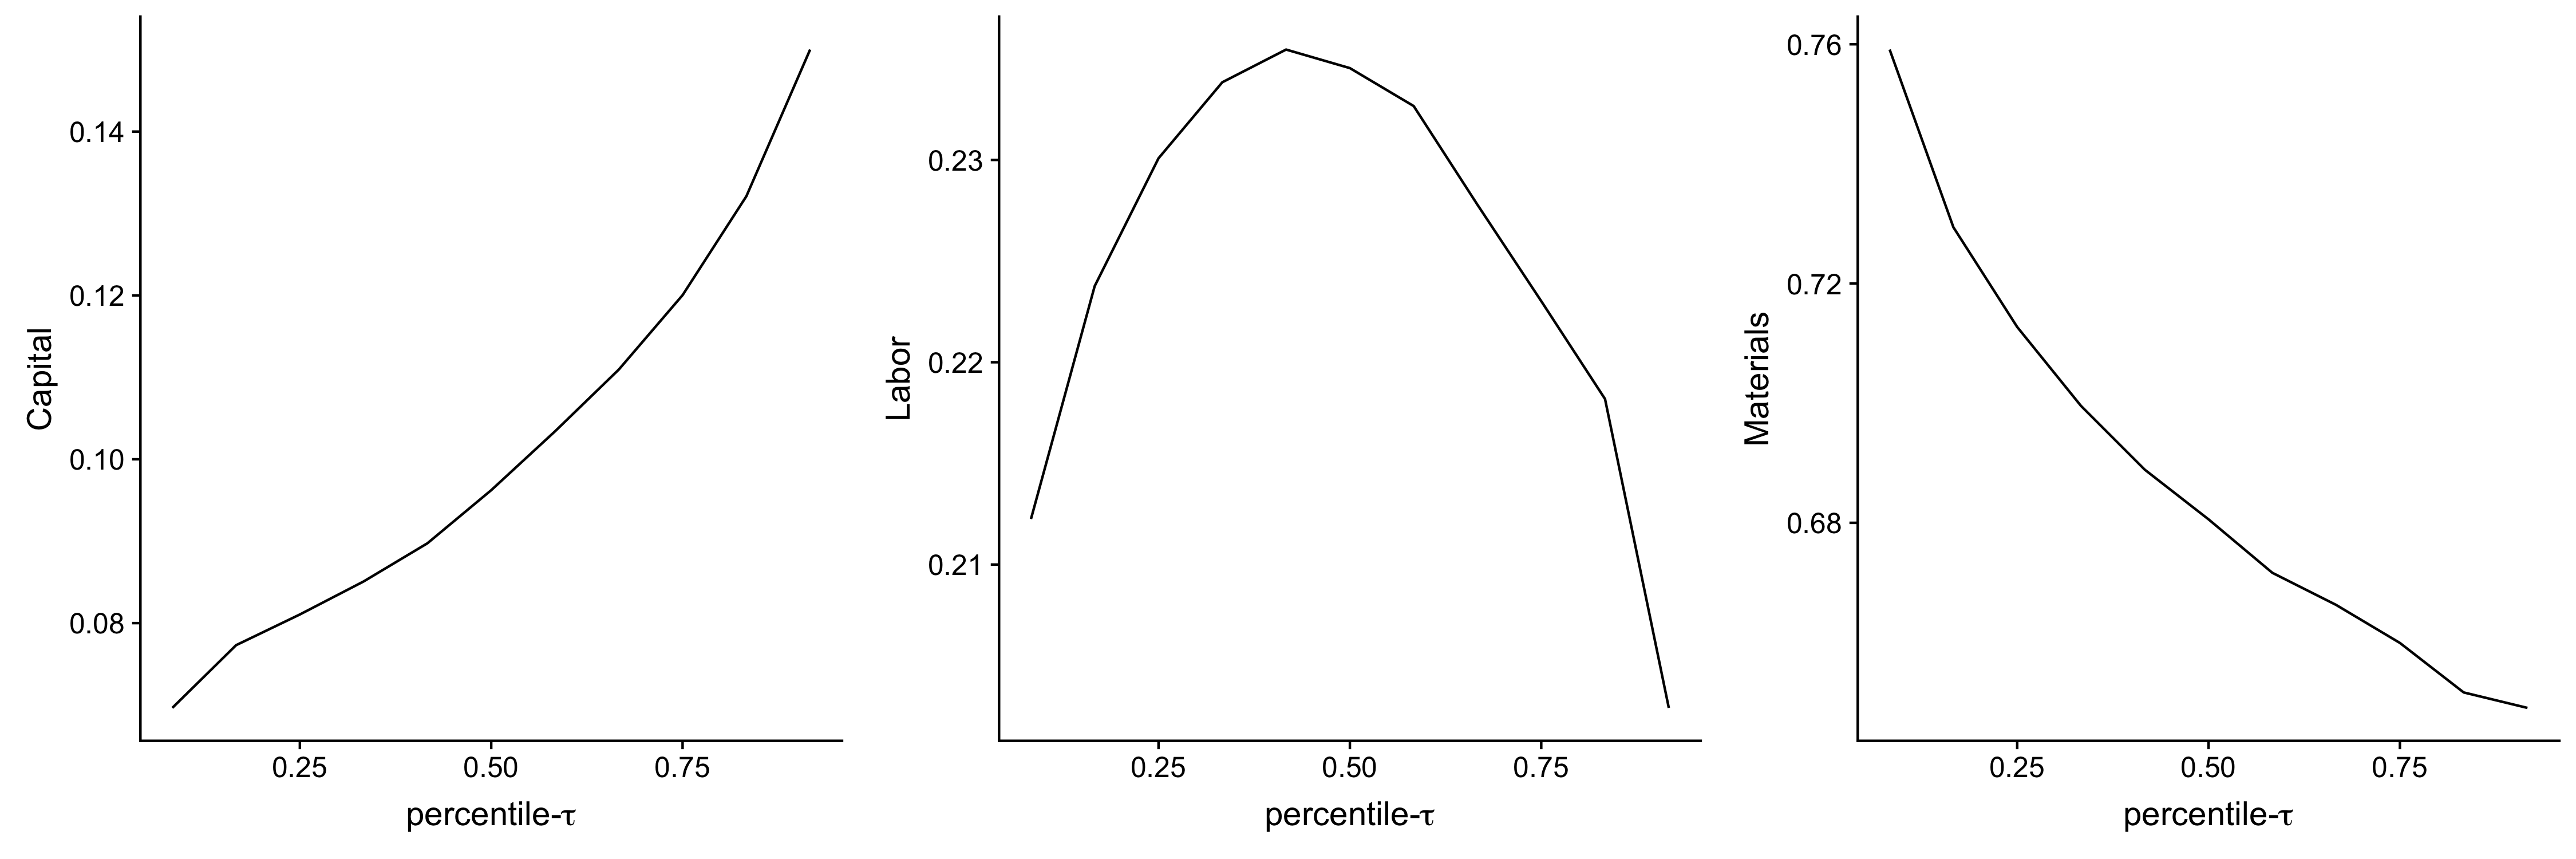
\includegraphics[width=15cm, height=5cm]{/Users/justindoty/Documents/Research/Dissertation/Nonlinear_Production_Function_QR/Code/Empirical/Investment/Plots/Elasticities/KLMAQME.png}
\label{klmaqme}
\end{figure} 

\begin{figure}[H]
\centering
\caption{Individual Output Elasticities}
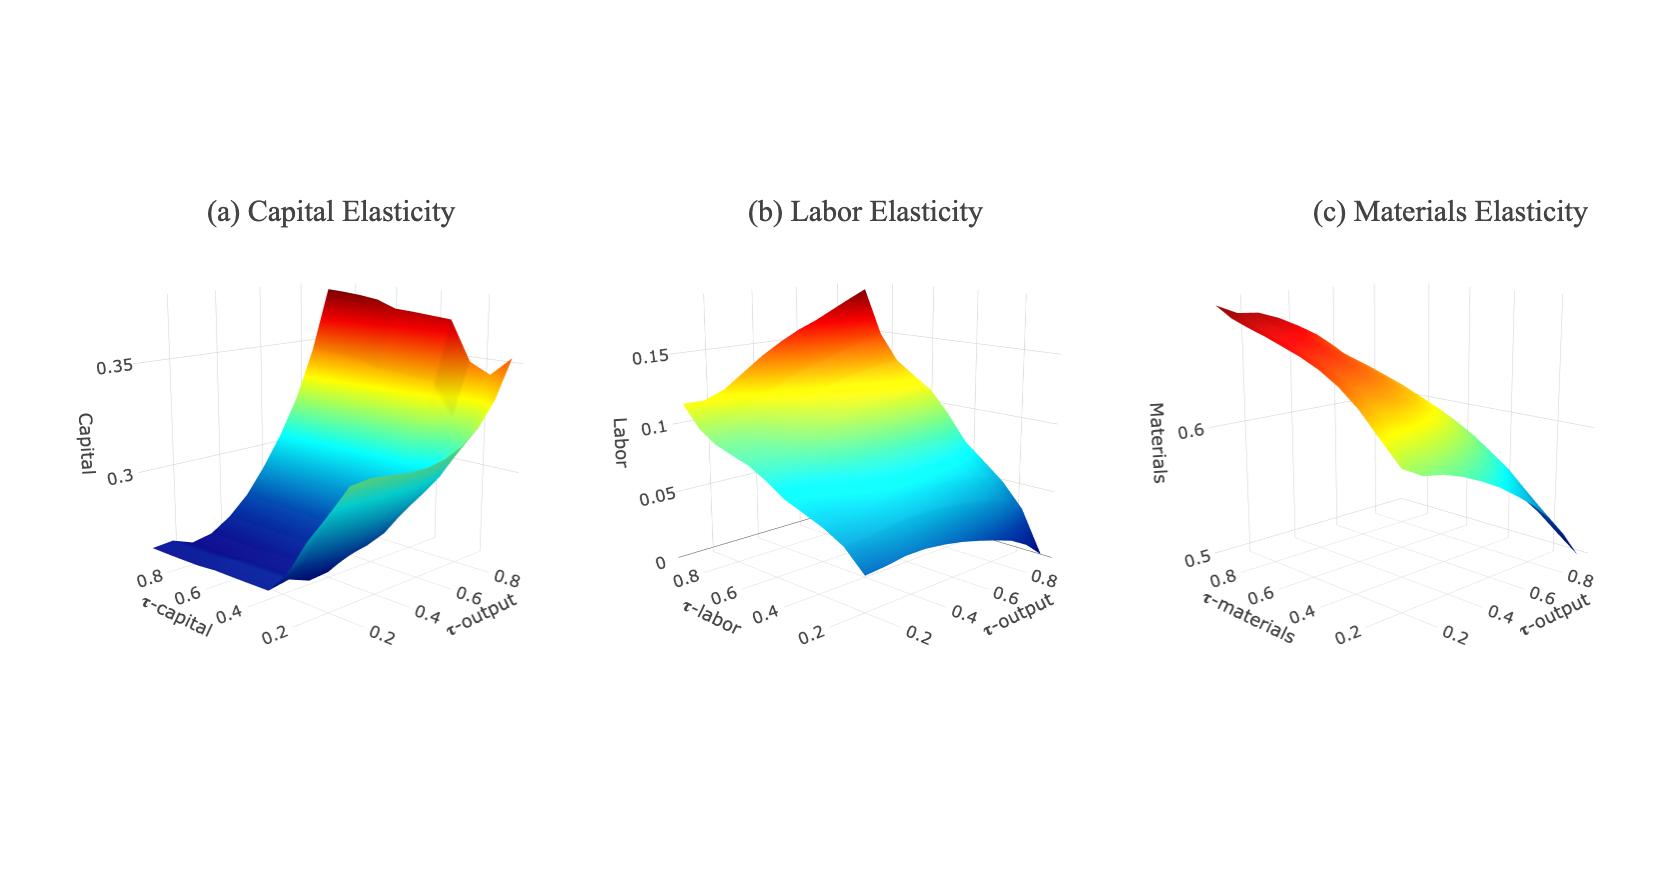
\includegraphics[width=15cm, height=5cm]{/Users/justindoty/Documents/Research/Dissertation/Nonlinear_Production_Function_QR/Code/Empirical/Investment/Plots/Elasticities/KLMIQME.png}
\label{klmiqme}
\end{figure} 

\begin{figure}[H]
\centering
\caption{Average Non-Hicks Neutral Elasticities}
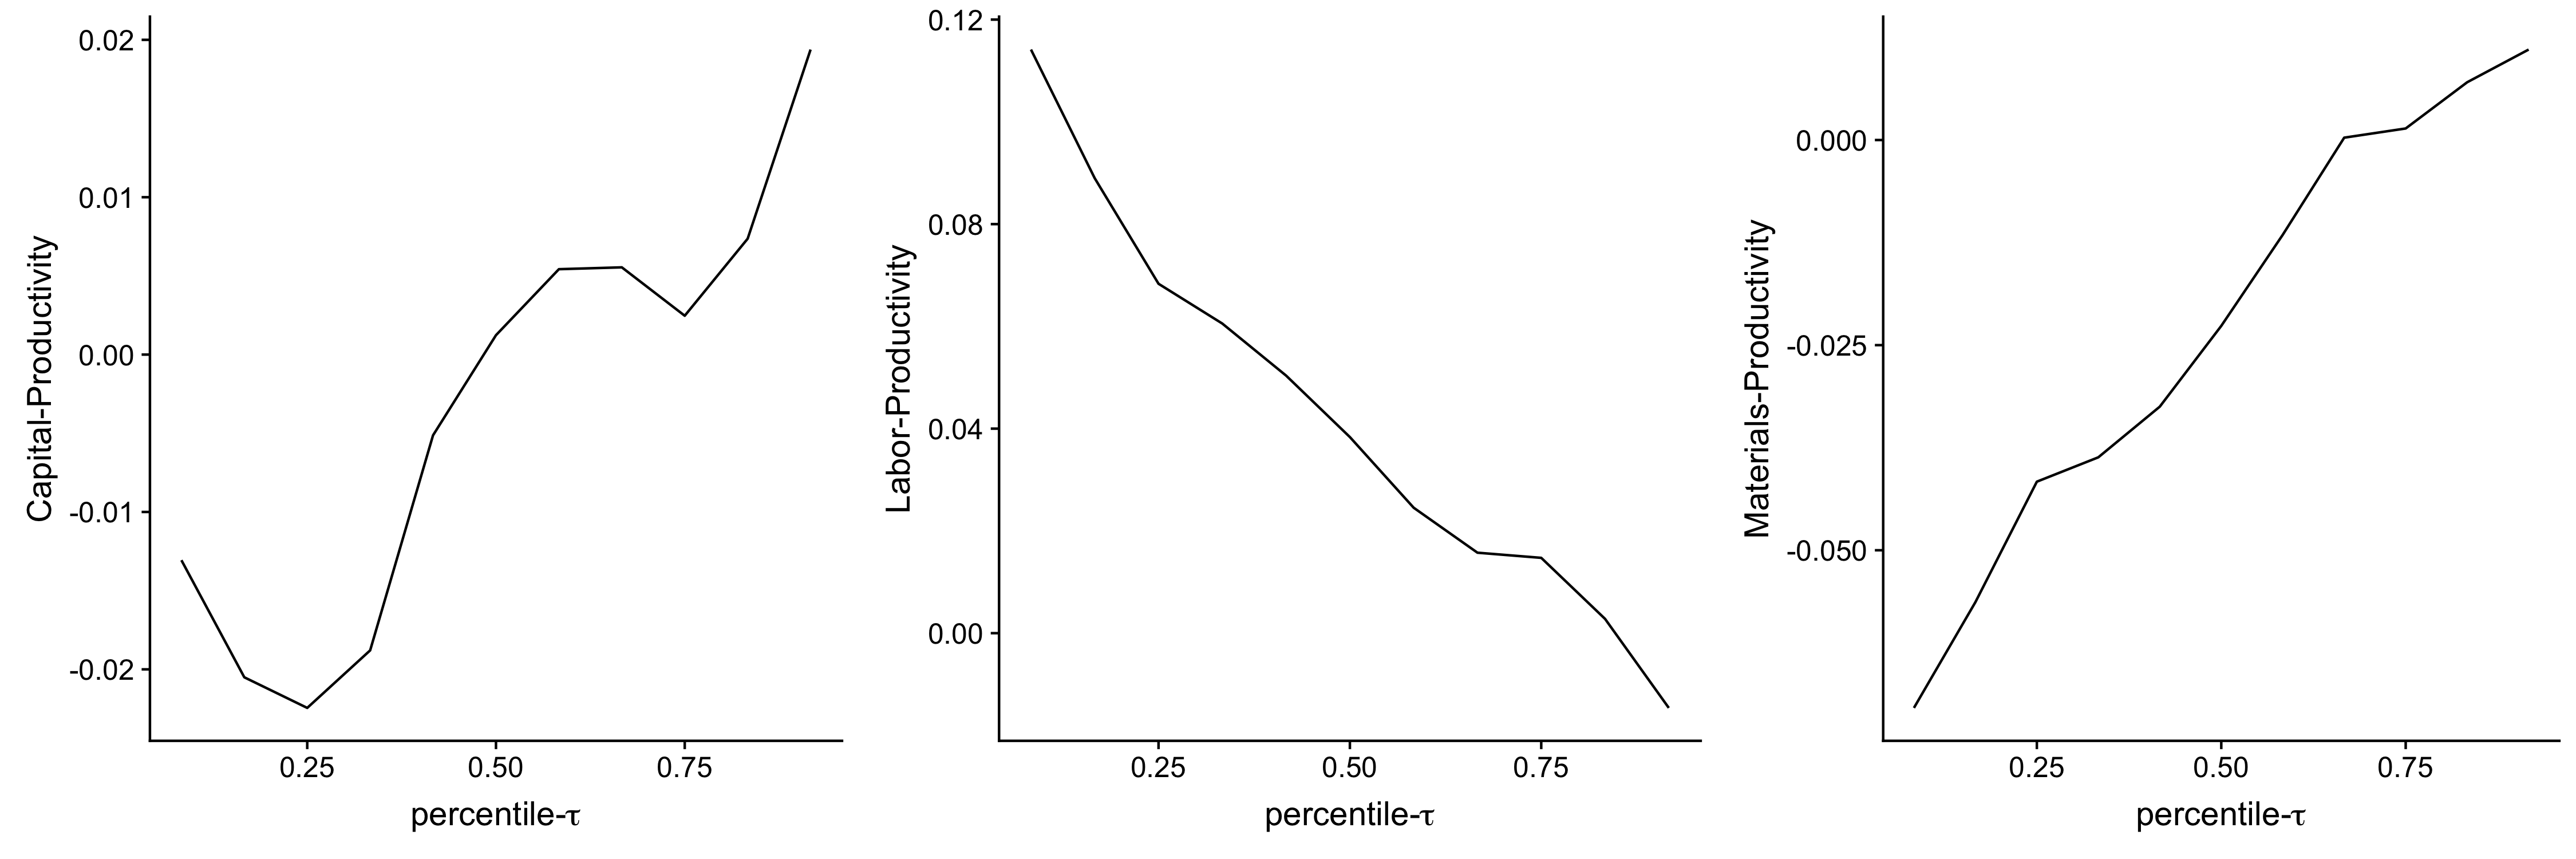
\includegraphics[width=15cm, height=5cm]{/Users/justindoty/Documents/Research/Dissertation/Nonlinear_Production_Function_QR/Code/Empirical/Investment/Plots/Elasticities/HKLMAQME.png}
\label{hklmaqme}
\end{figure} 

\begin{figure}[H]
\centering
\caption{Individual Non-Hicks Neutral Elasticities}
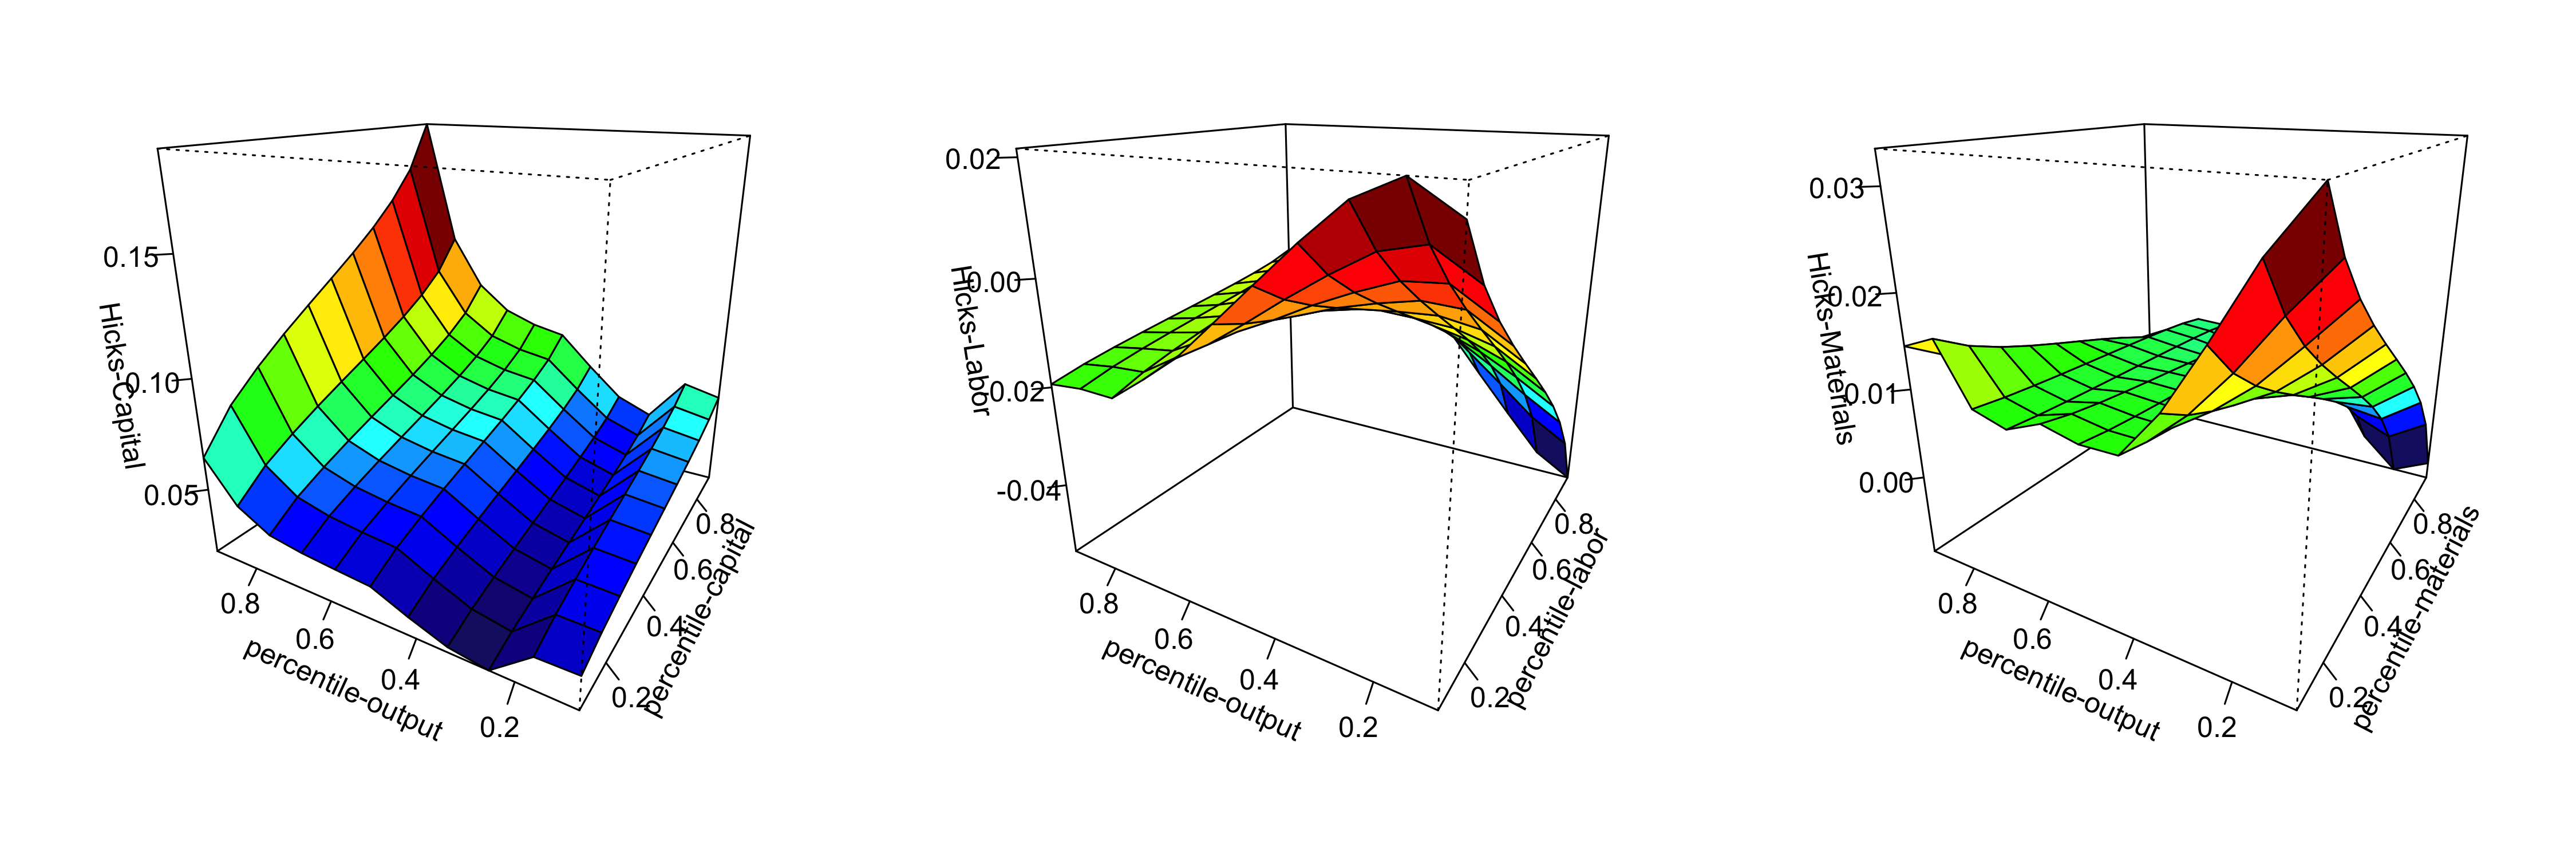
\includegraphics[width=15cm, height=5cm]{/Users/justindoty/Documents/Research/Dissertation/Nonlinear_Production_Function_QR/Code/Empirical/Investment/Plots/Elasticities/HKLMIQME.png}
\label{hklmiqme}
\end{figure}

\begin{figure}[H]
\centering
\caption{Productivity Persistence}
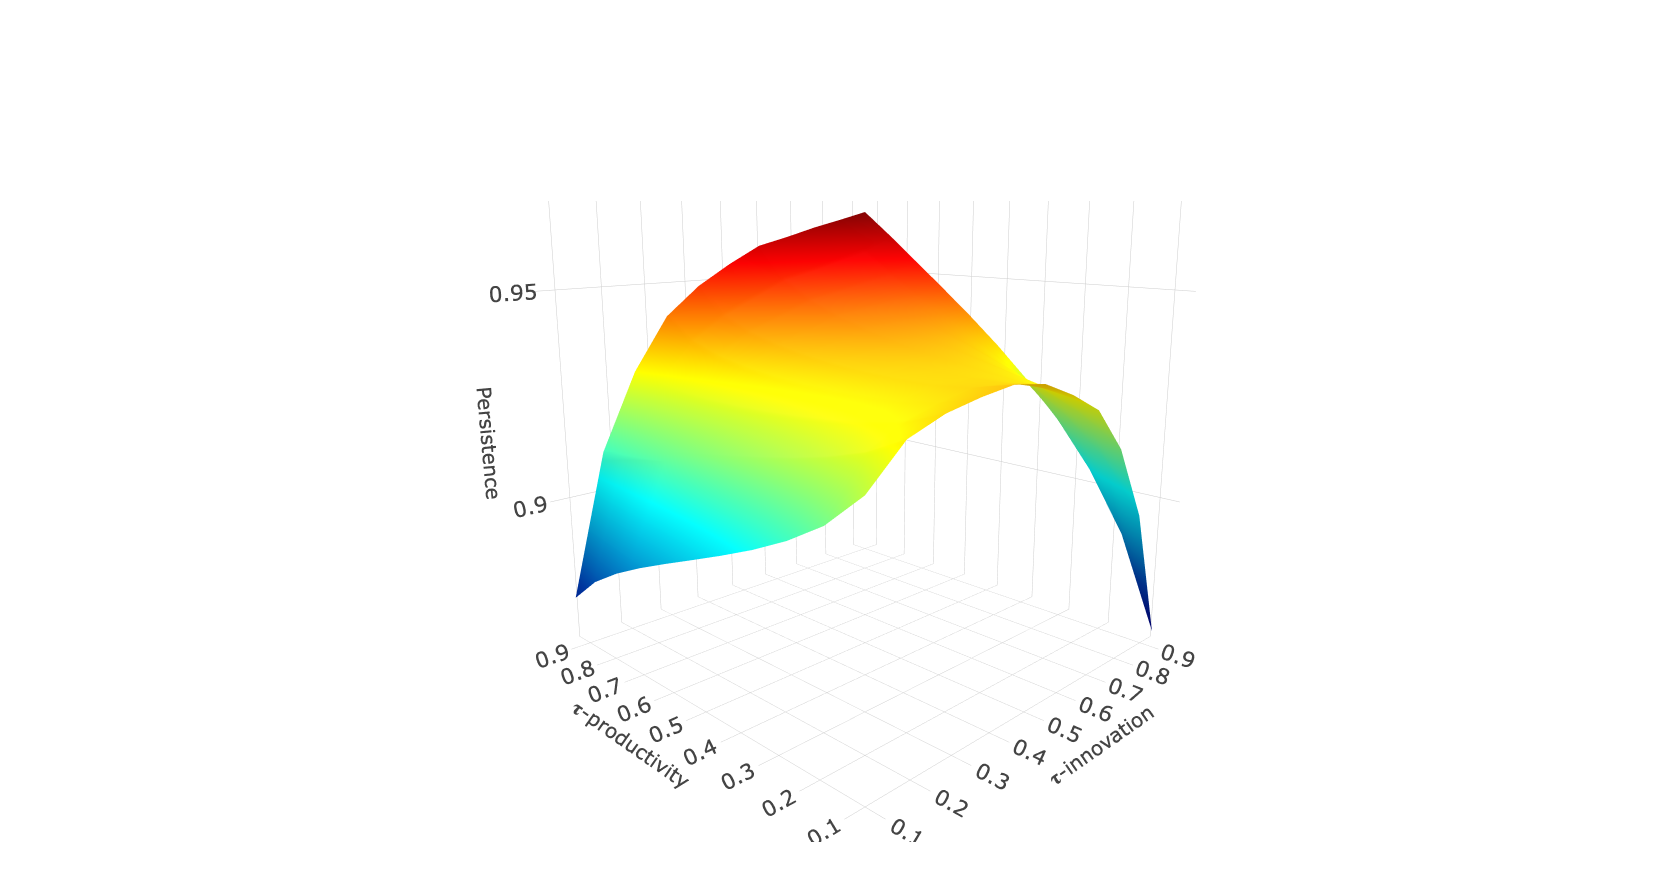
\includegraphics[width=9cm, height=9cm]{/Users/justindoty/Documents/Research/Dissertation/Nonlinear_Production_Function_QR/Code/Empirical/Investment/Plots/TFP/3dpers.png}
\label{pers}
\end{figure}

\begin{figure}[H]
\centering
\caption{Marginal Productivity of Inputs}
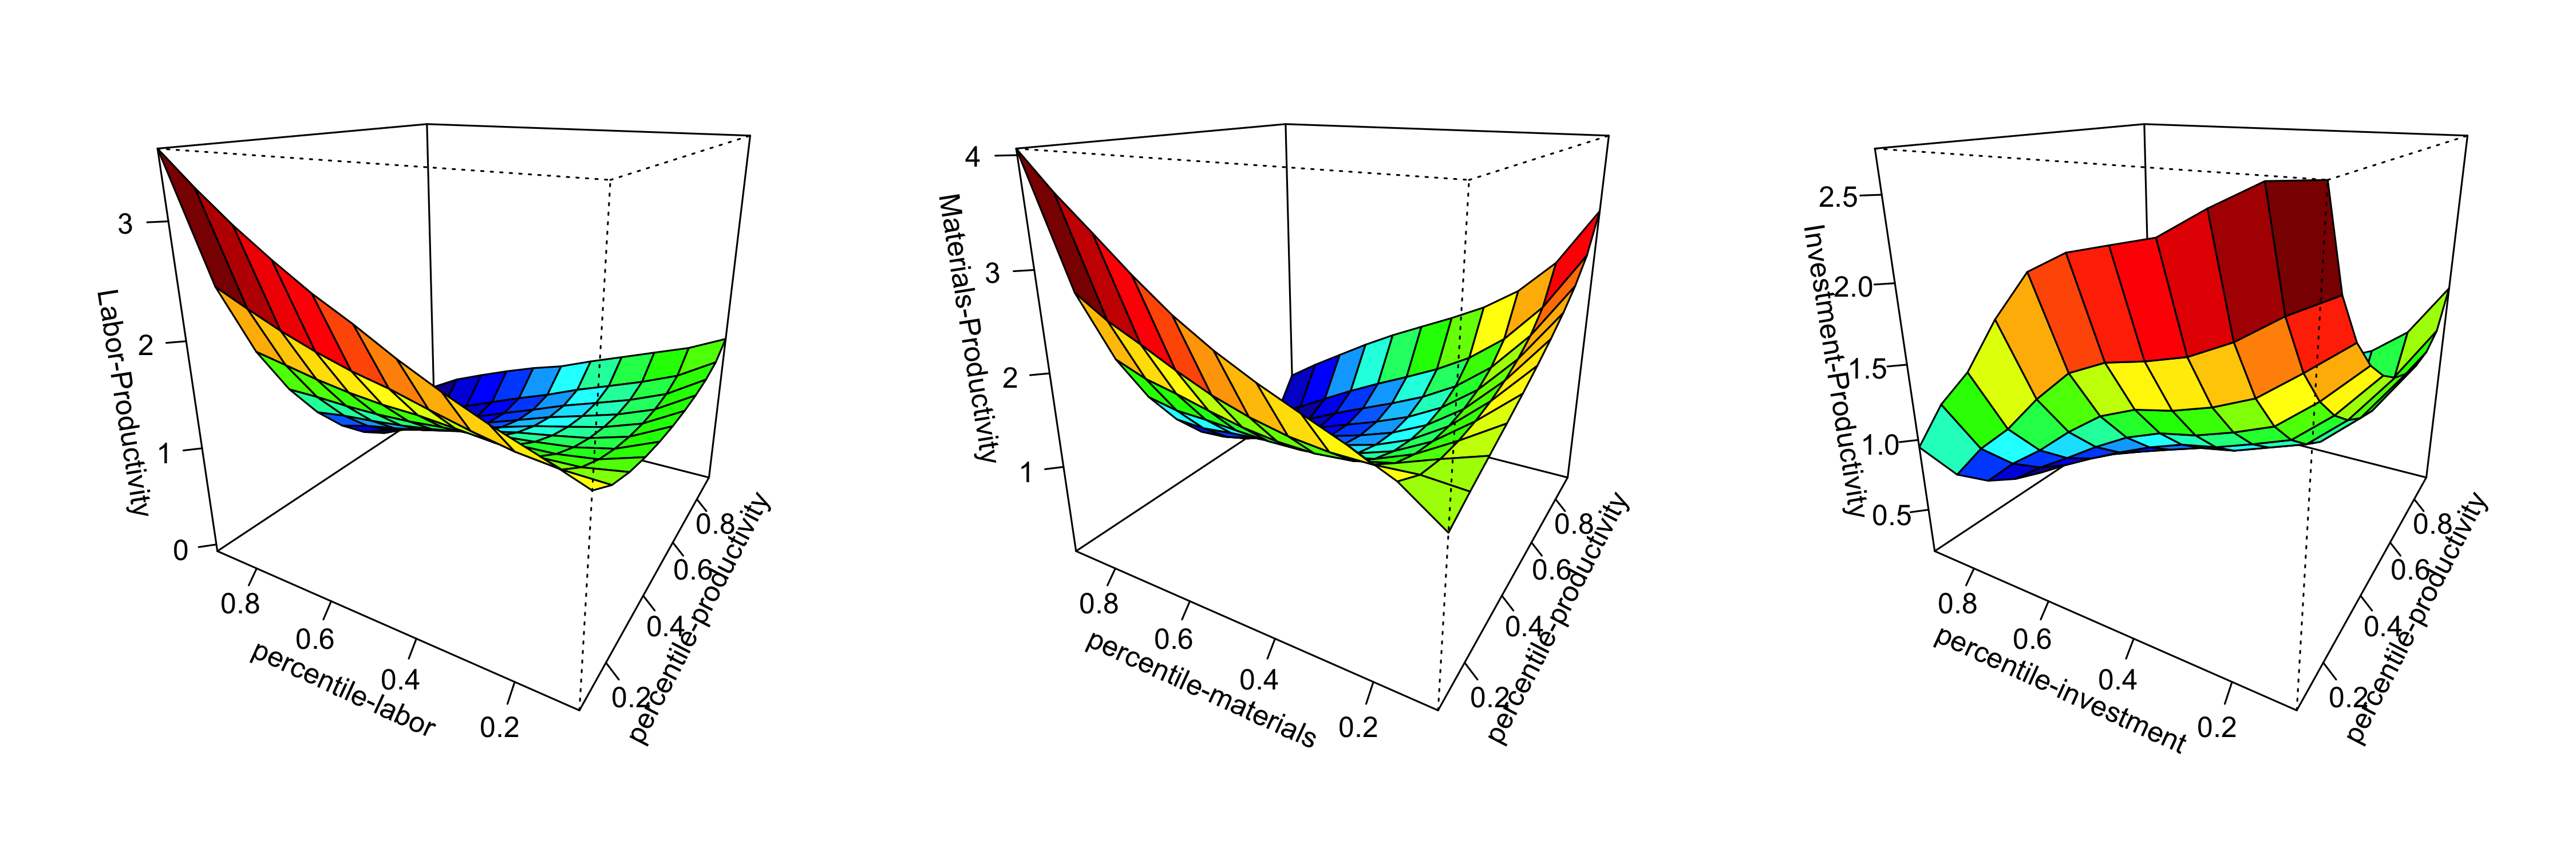
\includegraphics[width=12cm, height=5cm]{/Users/justindoty/Documents/Research/Dissertation/Nonlinear_Production_Function_QR/Code/Empirical/Investment/Plots/Inputs/LMIWPlot.png}
\label{lmiw}
\end{figure}

\begin{figure}[H]
\centering
\caption{Impulse Response of an Innovation Shock to Labor}
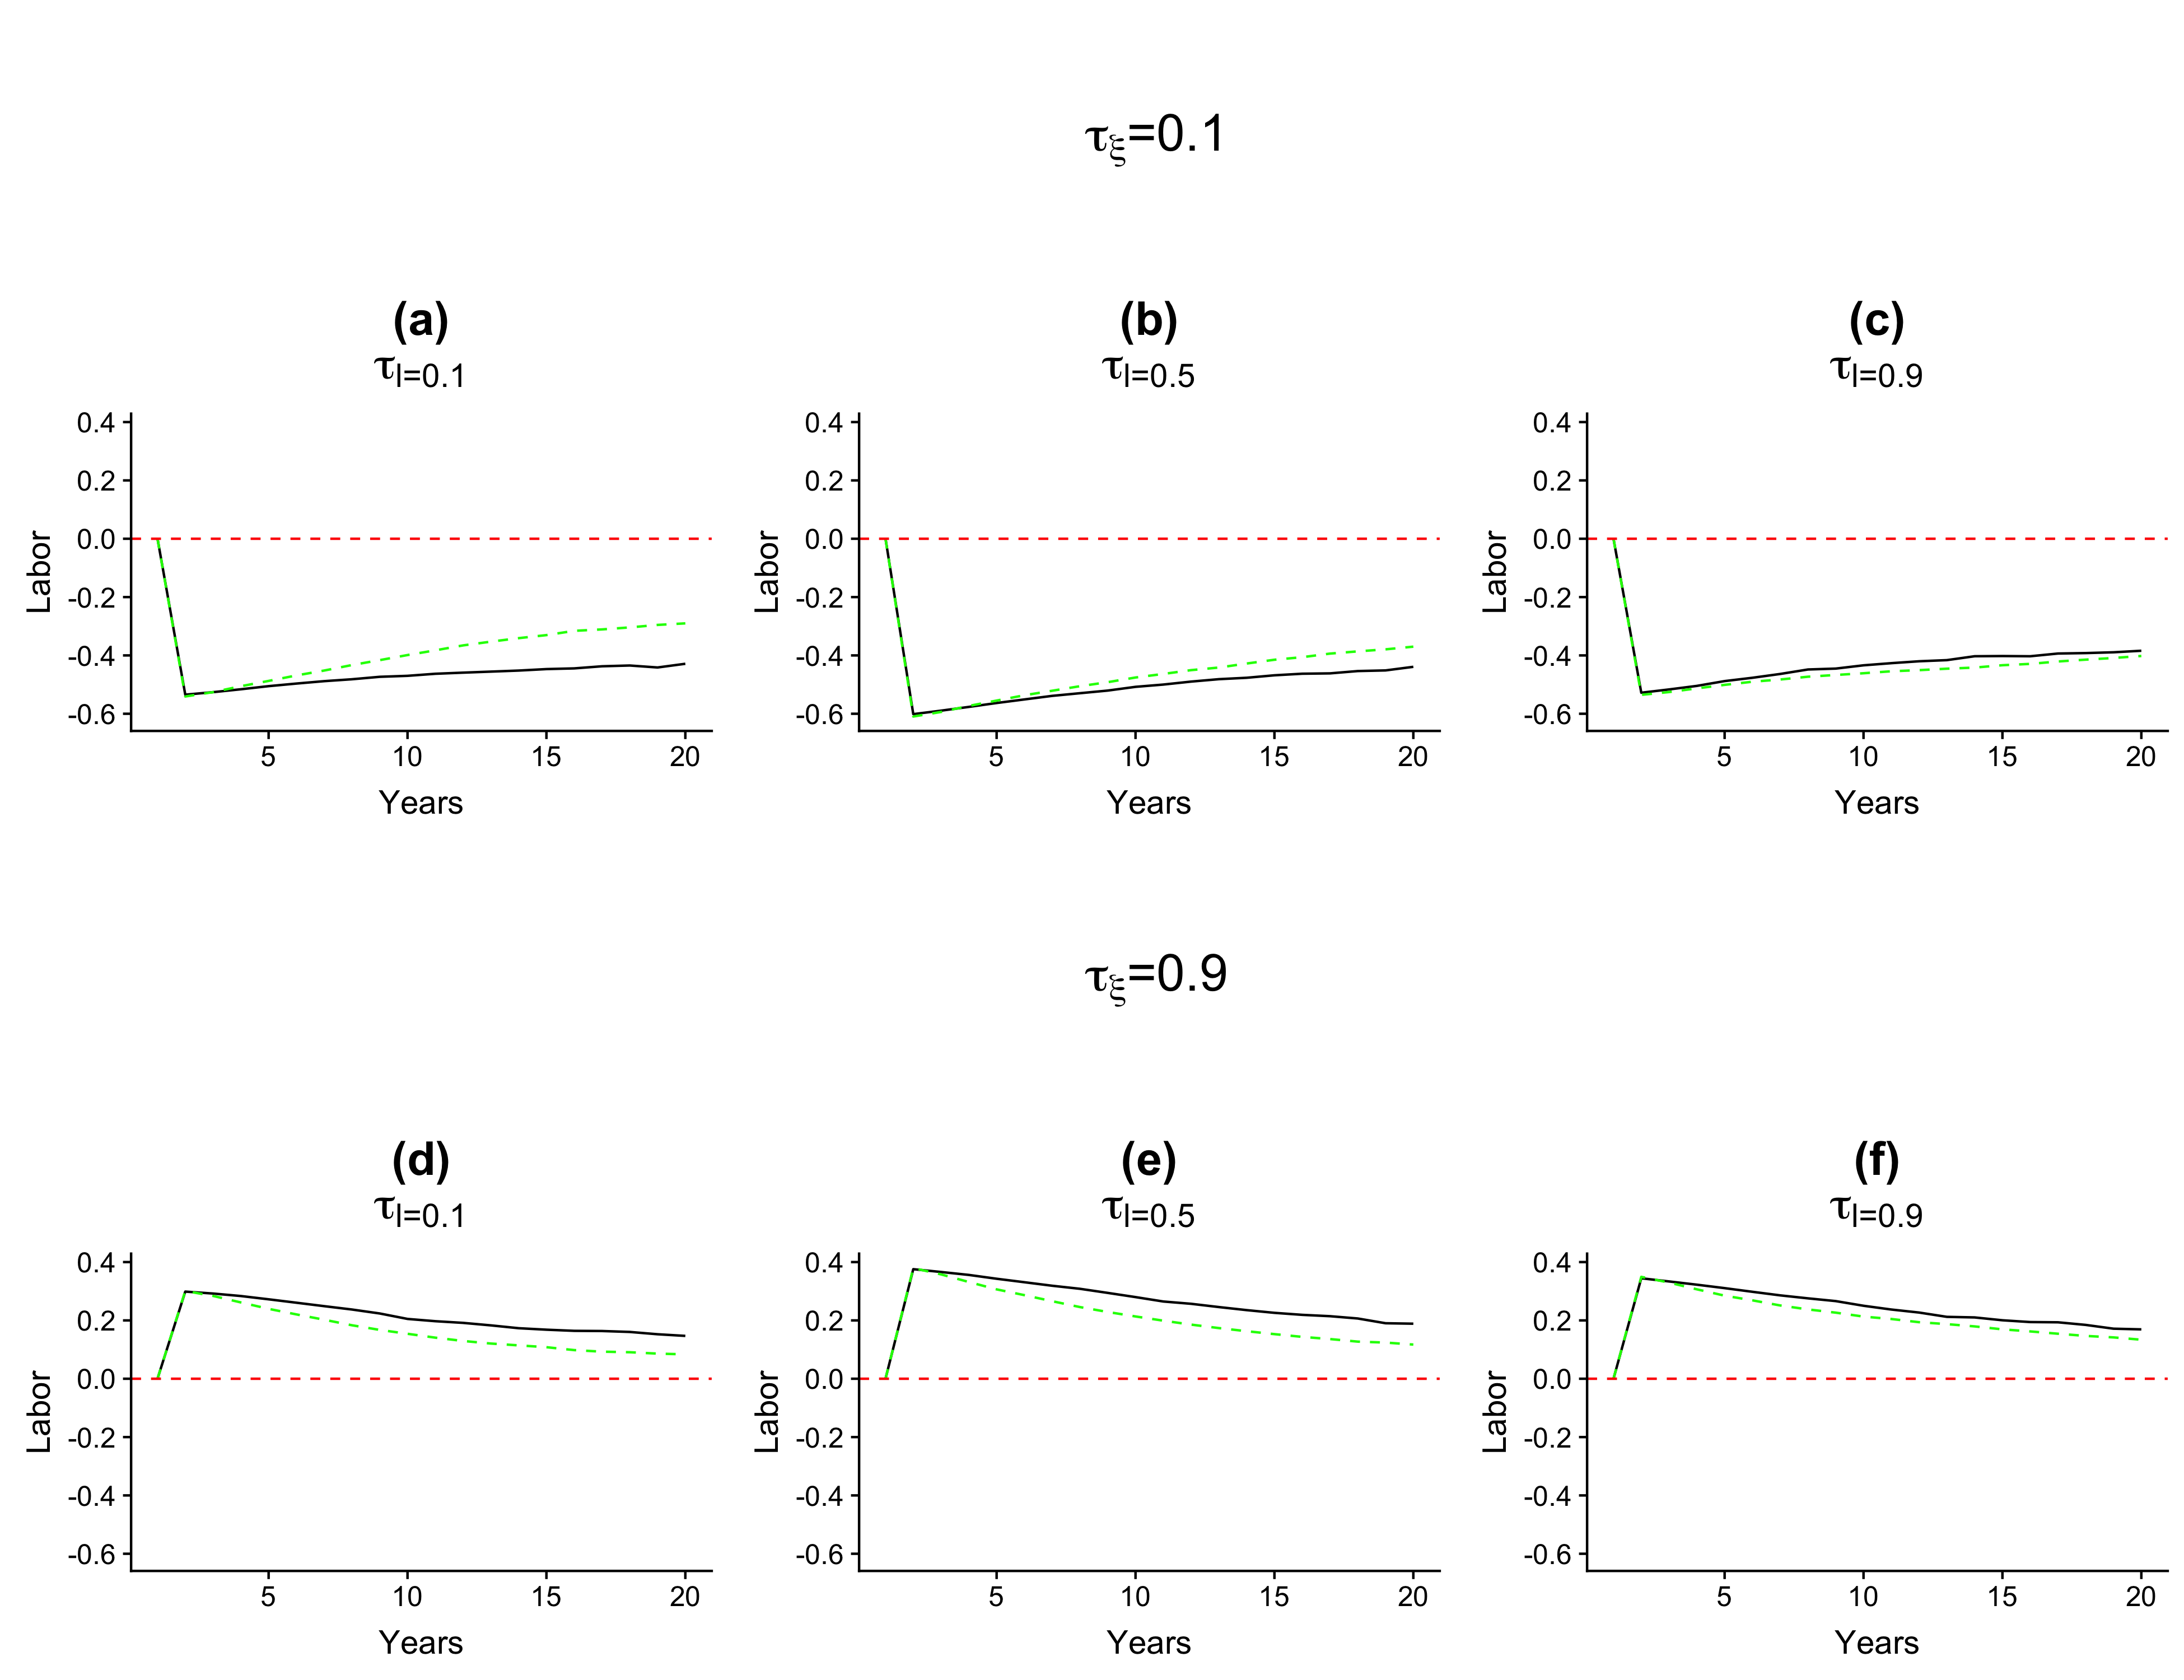
\includegraphics[width=11cm, height=15cm]{/Users/justindoty/Documents/Research/Dissertation/Nonlinear_Production_Function_QR/Code/Empirical/Investment/Plots/Inputs/impulseL.png}
\label{impulseL}
\end{figure}

\begin{figure}[H]
\centering
\caption{Impulse Response of an Innovation Shock to Materials}
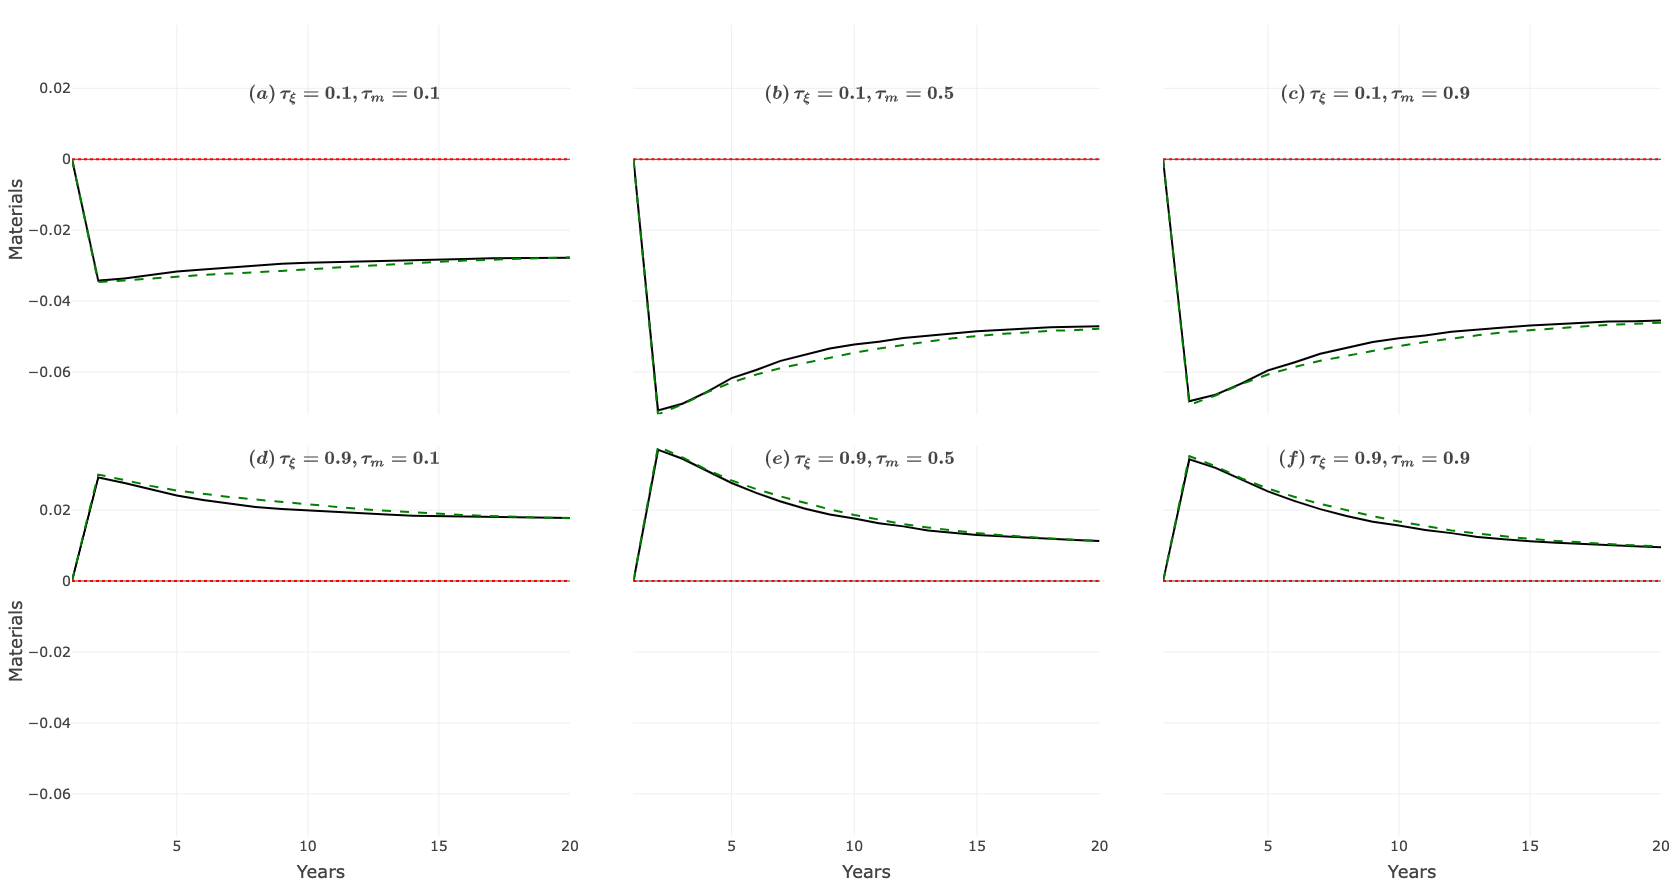
\includegraphics[width=11cm, height=15cm]{/Users/justindoty/Documents/Research/Dissertation/Nonlinear_Production_Function_QR/Code/Empirical/Investment/Plots/Inputs/impulseM.png}
\label{impulseM}
\end{figure}

\begin{figure}[H]
\centering
\caption{Impulse Response of an Innovation Shock to Capital}
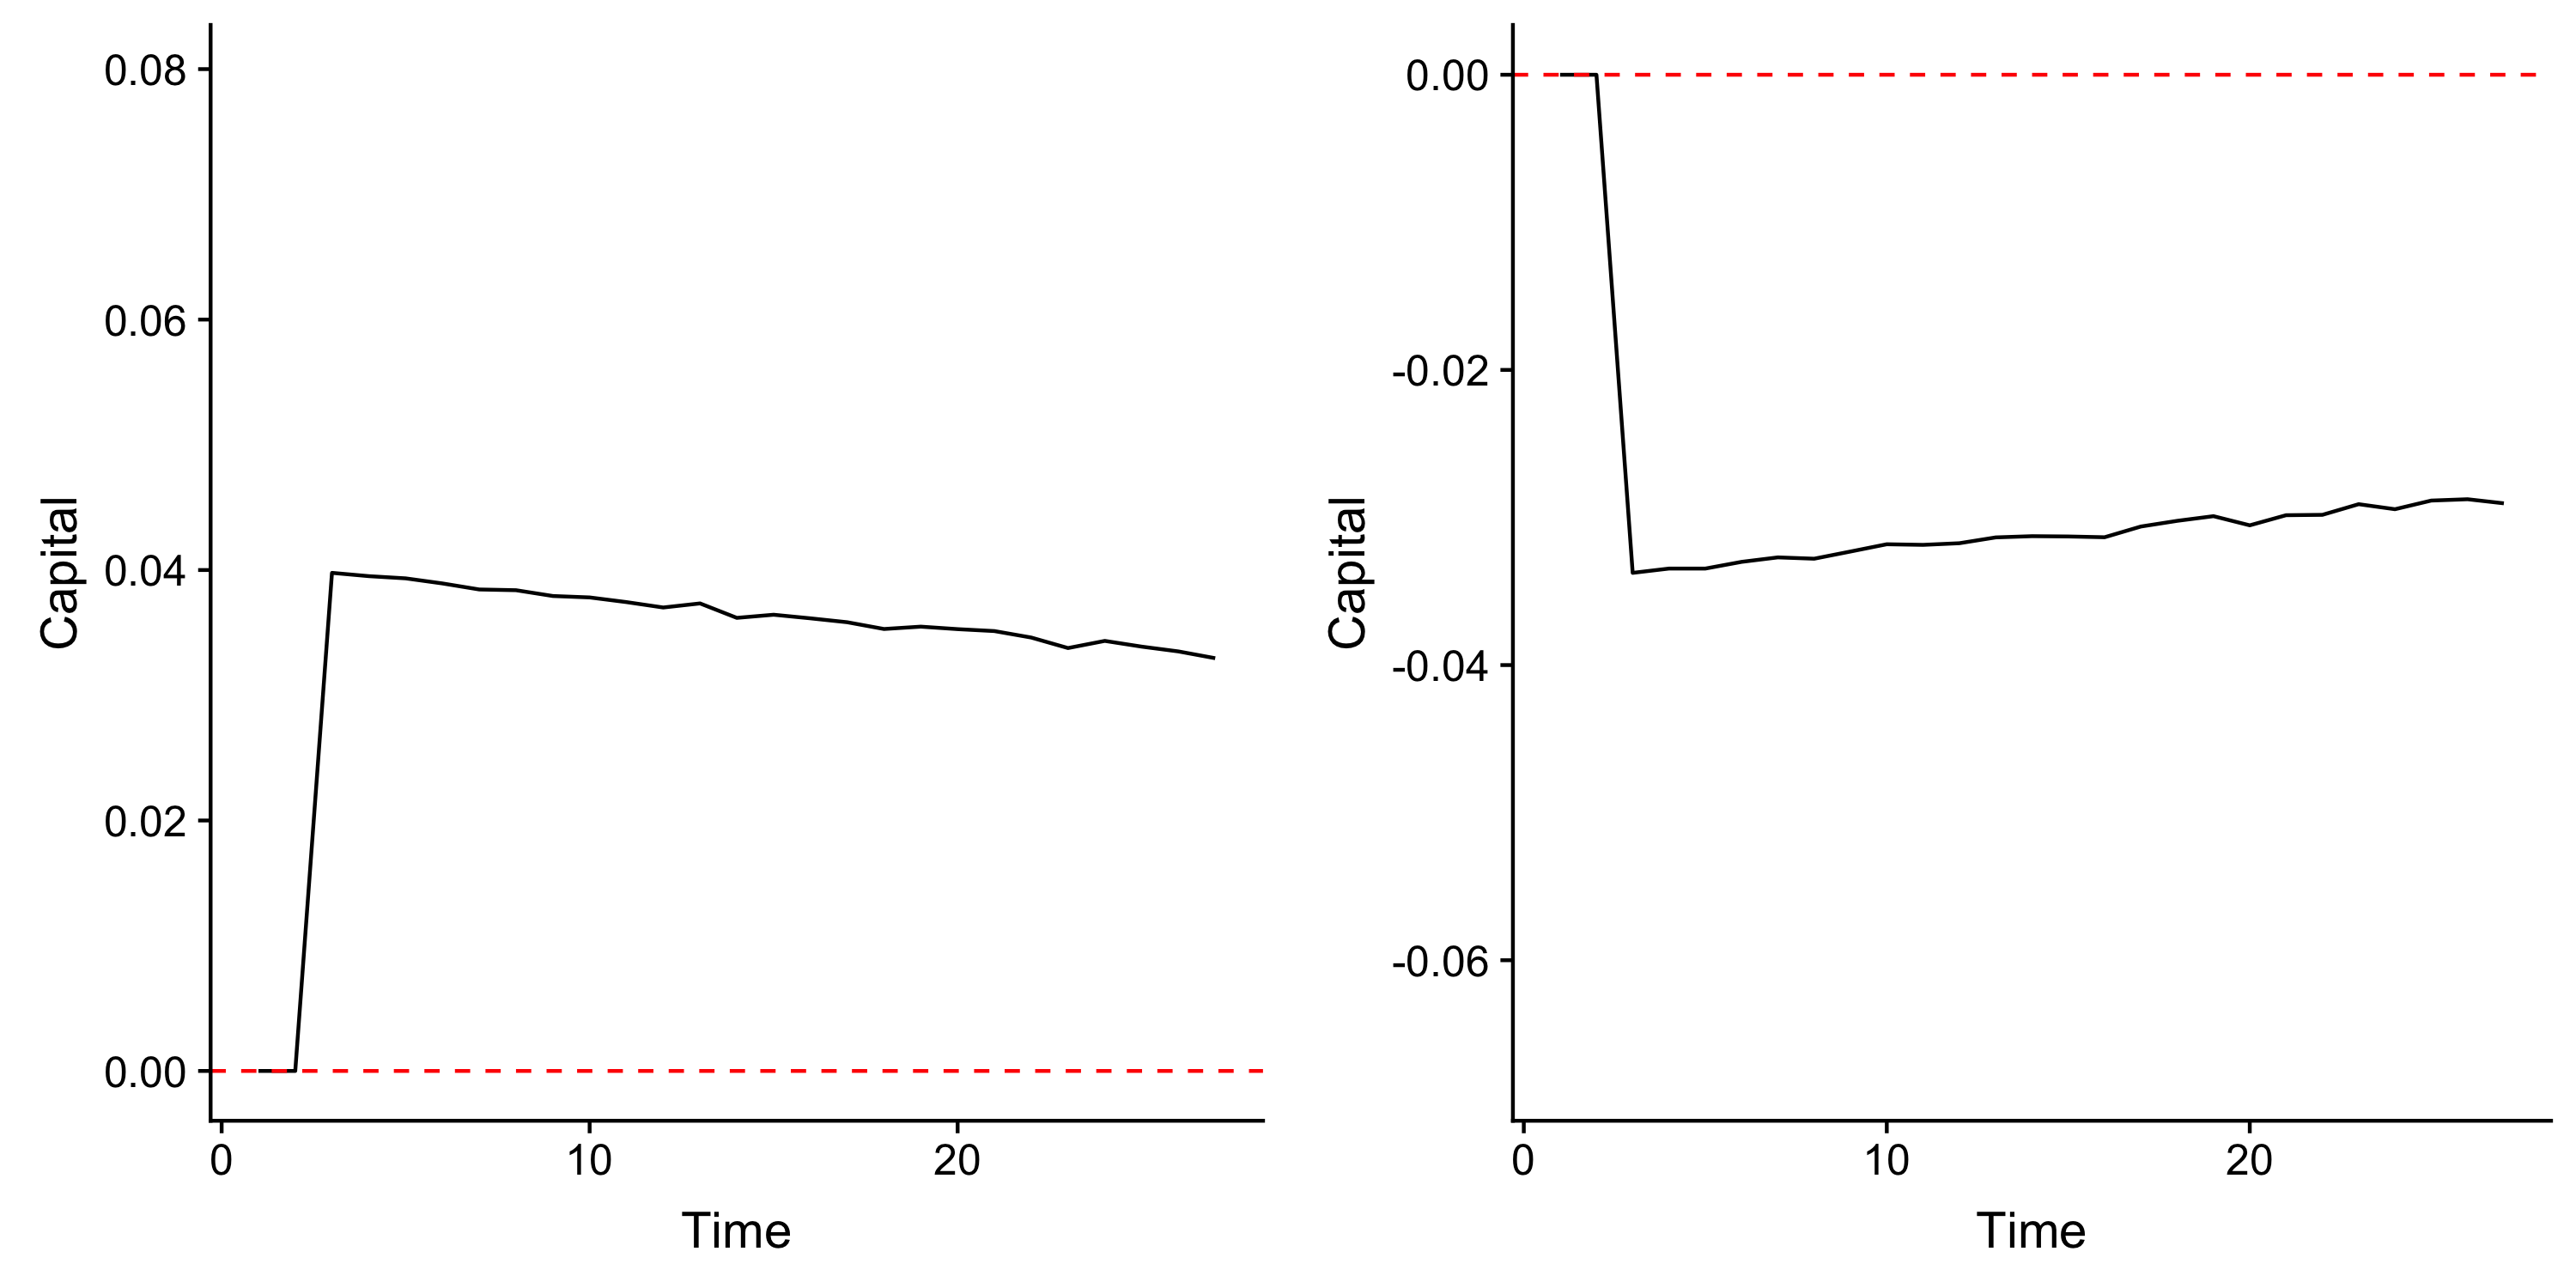
\includegraphics[width=11cm, height=15cm]{/Users/justindoty/Documents/Research/Dissertation/Nonlinear_Production_Function_QR/Code/Empirical/Investment/Plots/Inputs/impulseK.png}
\label{impulseK}
\end{figure}

\section{Conclusion} \label{conclusion}


\pagebreak
\newpage
\bibliographystyle{ecca.bst}
\bibliography{NL_PF_QR}

\pagebreak
\newpage

\appendix

                                          







\end{document}